\documentclass[oneside,final,14pt,a4paper]{extreport}

\usepackage{tempora} % Times New Roman alike font  

\usepackage{vmargin}
\setpapersize{A4}
\setmarginsrb{2.5cm}{2.0cm}{2.0cm}{2.0cm}{0pt}{10mm}{0pt}{13mm}
\usepackage{setspace}
\setstretch{1.5}
\usepackage{indentfirst}
\parindent=1.25cm

%%%%% ADDED TO SUPPORT TT BOLD FACES %%%%
\DeclareFontShape{OT1}{cmtt}{bx}{n}{<5><6><7><8><9><10><10.95><12><14.4><17.28><20.74><24.88>cmttb10}{}
\renewcommand{\ttdefault}{pcr}
%%%%% END %%%%%%%%%%%%%%%%%%%%%%%%%%%%%%% 

\usepackage{atbegshi,picture}
\usepackage[T1,T2A]{fontenc}
\usepackage[utf8]{inputenc}

\usepackage[english]{babel}
\usepackage[backend=biber,style=ieee,autocite=inline]{biblatex}
\bibliography{ref.bib}
\DefineBibliographyStrings{english}{%
  bibliography = {References},}
\usepackage{blindtext}

\usepackage{pdfpages}
\newenvironment{bottompar}{\par\vspace*{\fill}}{\clearpage}
\usepackage{amsmath,amsfonts}
\usepackage{url}
\usepackage{amsthm}
\newtheorem{theorem}{Theorem}
\newtheorem{corollary}{Corollary}
\newtheorem{lemma}{Lemma}
\newtheorem{proposition}{Proposition}
\theoremstyle{definition}
\newtheorem{definition}{Definition}
\theoremstyle{remark}
\newtheorem*{remark}{Remark}
\theoremstyle{remark}
\newtheorem*{example}{Example}

\usepackage{float}
\usepackage{graphicx}
\graphicspath{{figs/}} %path to images
\usepackage{array}
\usepackage{multirow,array}
\usepackage{caption}
\usepackage{subcaption}
\usepackage{hyperref}
\hypersetup{colorlinks=true, linkcolor=black, citecolor=black}
\usepackage{paralist}
\usepackage{listings}
\usepackage{zed-csp}
\usepackage{fancyhdr}
\usepackage{csquotes}
\usepackage{xcolor}

% Listings configuration for Go code
\definecolor{codegreen}{rgb}{0,0.6,0}
\definecolor{codegray}{rgb}{0.5,0.5,0.5}
\definecolor{codepurple}{rgb}{0.58,0,0.82}
\definecolor{backcolour}{rgb}{0.95,0.95,0.92}
\definecolor{commentred}{rgb}{0.6,0,0}

\lstdefinestyle{mystyle}{
    backgroundcolor=\color{backcolour},
    commentstyle=\color{commentred}\itshape,
    keywordstyle=\color{blue}\bfseries,
    numberstyle=\tiny\color{codegray},
    stringstyle=\color{codepurple},
    basicstyle=\footnotesize\ttfamily,
    breakatwhitespace=false,
    breaklines=true,
    captionpos=b,
    keepspaces=true,
    numbers=left,
    numbersep=5pt,
    showspaces=false,
    showstringspaces=false,
    showtabs=false,
    tabsize=4,
    frame=single,
    framerule=0.5pt,
    rulecolor=\color{codegray},
    xleftmargin=2em,
    xrightmargin=2em,
    aboveskip=0.5em,
    belowskip=0.5em,
    language=Go
}

\lstset{style=mystyle}

% Declare Go language
\lstdefinelanguage{Go}{
  morekeywords={[1]package,import,func,type,struct,return,defer,panic,
    recover,select,var,const,iota,for,range,if,else,switch,case,fallthrough,
    goto,break,continue,go,chansend,sqsend,select,chan,map,interface,
    default,go,goto},
  morekeywords={[2]bool,byte,complex64,complex128,error,float32,float64,
    int,int8,int16,int32,int64,rune,string,uint,uint8,uint16,uint32,uint64,uintptr},
  morekeywords={[3]true,false,nil,new,make,append,cap,close,complex,
    copy,delete,imag,len,make,new,panic,print,println,real,recover},
  sensitive=true,
  morecomment=[l]{//},
  morecomment=[s]{/*}{*/},
  morestring=[b]",
  morestring=[b]`,
  morestring=[b]'
}

% Declare Bash language
\lstdefinelanguage{bash}{
  morekeywords={if,then,else,fi,for,do,done,while,case,esac,function,
    select,in,until,elif,export,unset,local,read,return,exit,break,continue,
    shift,let,set,echo,printf,test,eval,trap,wait,exec,cd,pwd,ls,cp,mv,rm,
    mkdir,rmdir,cat,head,tail,grep,sed,awk,cut,sort,uniq,wc,find,xargs,
    curl,wget,git,docker,kubectl,hey,go},
  sensitive=false,
  morecomment=[l]{\#},
  morecomment=[s]{\#<}{>},
  morestring=[b]",
  morestring=[b]',
  morestring=[b]`
}

% Declare YAML language
\lstdefinelanguage{yaml}{
  keywords={true,false,null,y,n},
  keywordstyle=\color{blue}\bfseries,
  basicstyle=\footnotesize\ttfamily,
  sensitive=false,
  comment=[l]{\#},
  morecomment=[l]{\#},
  morestring=[b]',
  morestring=[b]",
  showstringspaces=false
}
% \usepackage{anyfontsize}
% \usepackage{mathptmx}
% \usepackage{t1enc}

\usepackage{chngcntr}
\usepackage{upgreek}
\usepackage{bm}
\usepackage{booktabs}
\usepackage{multirow}
\usepackage{longtable}
\usepackage{tabularx}
\usepackage[font=singlespacing, labelfont=bf]{caption}
\usepackage{ragged2e}
\justifying
%Hints
\newcommand\pic[1]{(Fig.\ \ref{#1})} %Ref on figure
\newcommand\tab[1]{(Tab.\ \ref{#1})} %Ref on table

\setlength{\headheight}{32.0976pt}
\usepackage{enumitem}
\newlist{inlinelist}{enumerate*}{1}
\setlist*[inlinelist,1]{%
  label= (\arabic*),
}

% \setcounter{secnumdepth}{4}
\captionsetup[table]{labelfont={normalfont}, name={TABLE}, labelsep={newline}, justification=centering}
\setlength{\parindent}{1.25cm} 
\DeclareCaptionLabelSeparator{figSep}{.\quad}
\captionsetup[figure]{labelfont={normalfont}, name={Fig.}, labelsep=period}
\counterwithin{figure}{chapter}

% \usepackage{titlesec}
% \titleformat{\section}[hang]{\fontsize{20}{24}\selectfont\filcenter}{\Roman{section}}{1em}{}
% \titleformat{\subsection}[hang]{\itshape}{\Alph{subsection}.}{1em}{}[]
% \titleformat{\subsubsection}[runin]{\itshape}{\arabic{subsubsection})}{1em}{}[$:$]
% \titlespacing{\subsubsection}{1em}{1em}{1em}
% \titleformat{\paragraph}[runin]{\itshape}{\alph{paragraph})}{1em}{}[$:$\quad]
% \titlespacing{\paragraph}{2em}{1em}{1em}

\usepackage{placeins} % for \FloatBarrier

\pagestyle{fancyplain}

% remember section title
\renewcommand{\chaptermark}[1]%
	{\markboth{\chaptername~\thechapter~--~#1}{}}

% subsection number and title
\renewcommand{\sectionmark}[1]%
	{\markright{\thesection\ #1}}

\rhead[\fancyplain{}{\bf\leftmark}]%
      {\fancyplain{}{\bf\thepage}}
\lhead[\fancyplain{}{\bf\thepage}]%
      {\fancyplain{}{\bf\rightmark}}
\cfoot{} %bfseries


\newcommand{\dedication}[1]
   {\thispagestyle{empty}
     
   \begin{flushleft}\raggedleft#1\end{flushleft}
}

\begin{document}

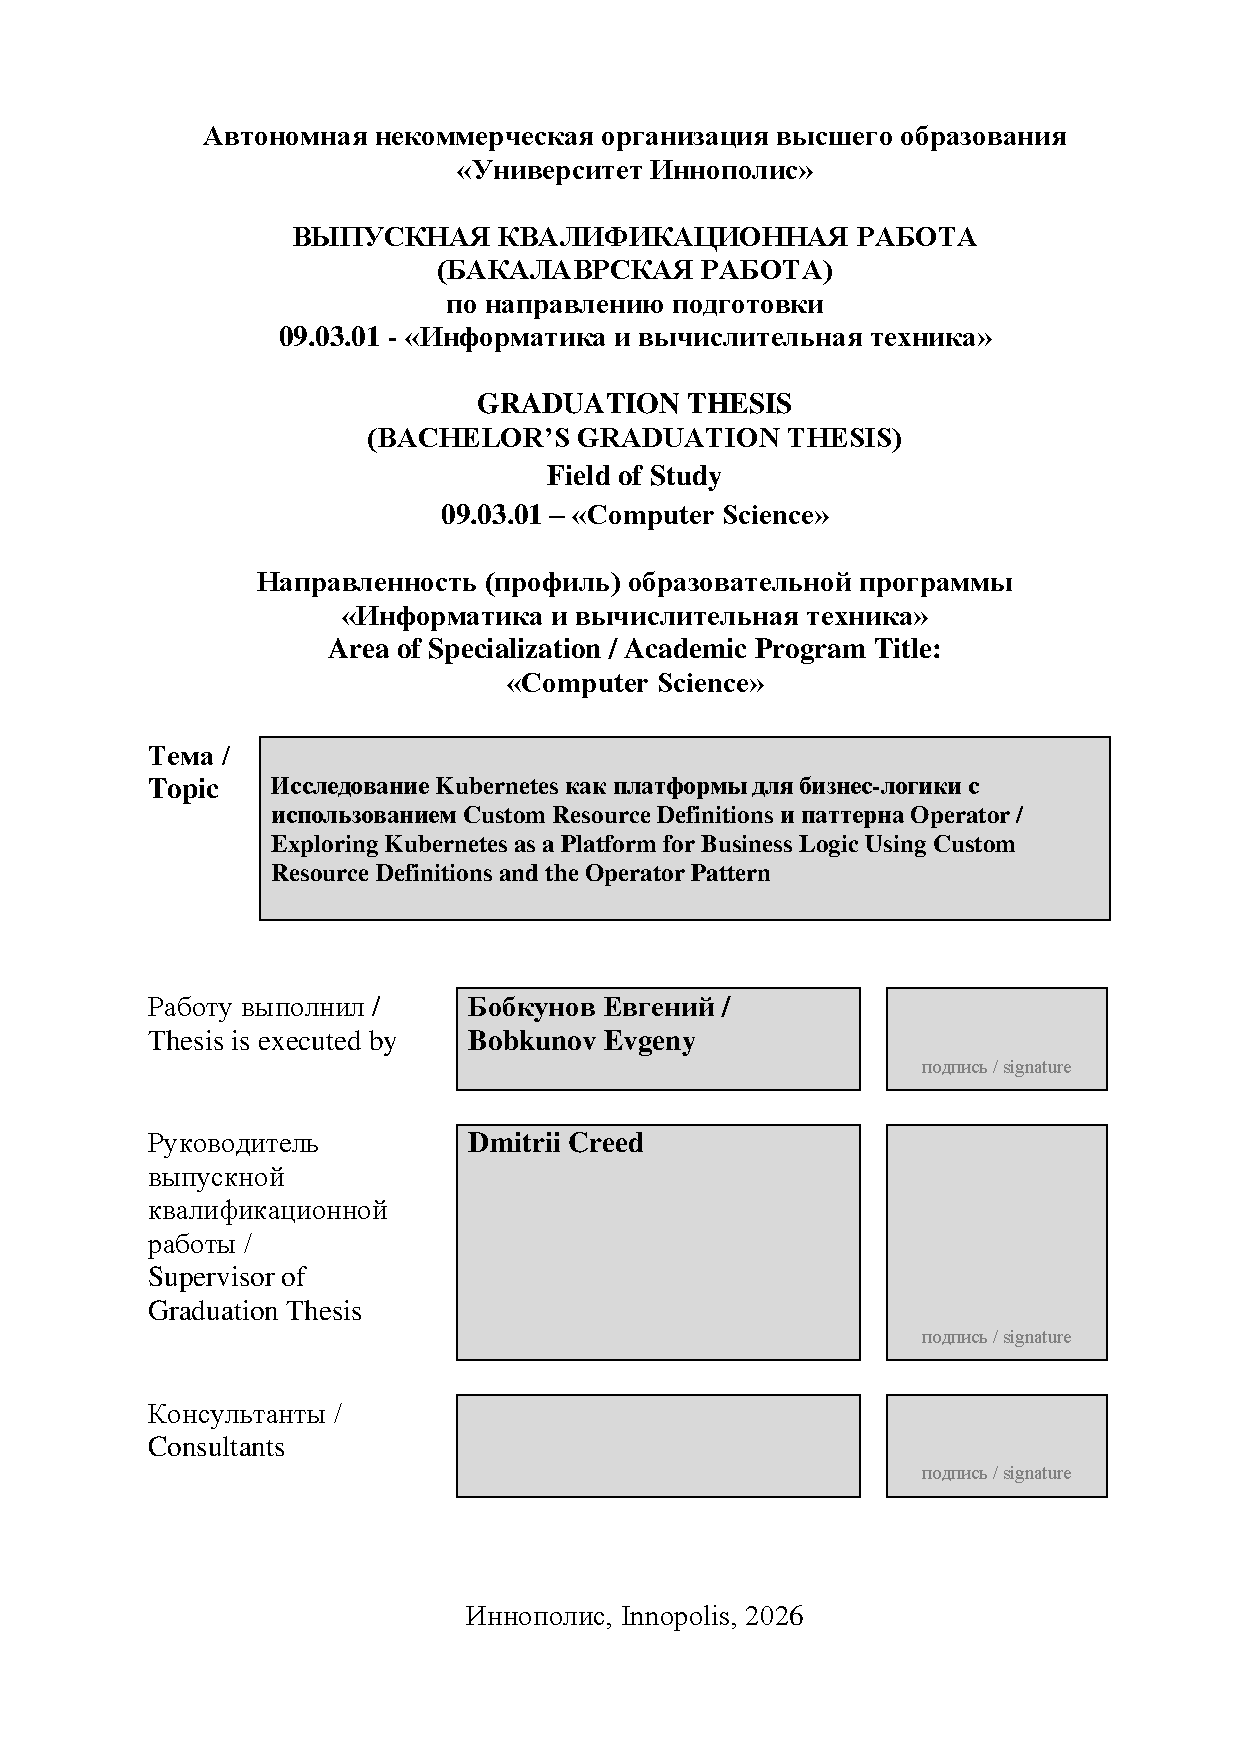
\includepdf[pages=-, offset=72 -72, pagecommand={\thispagestyle{empty}}]{title.pdf}
\tableofcontents
%\listoftables
%\listoffigures
\newpage


\begin{abstract}

This thesis explores the applicability of Kubernetes as a platform for implementing business logic using Custom Resource Definitions (CRDs) and the Operator pattern. While Kubernetes has become the de facto standard for container orchestration, its potential as a business logic platform remains understudied.

Two functionally equivalent billing systems were designed and implemented: (1) a traditional Go backend with REST API and PostgreSQL database, and (2) a Kubernetes Operator with CRDs and reconcile-based control loop. Both systems implement identical business logic (billing plan management, subscription lifecycle, recurring billing, expiration handling) but differ fundamentally in architecture, state management, and execution model.

Comprehensive evaluation was conducted across multiple dimensions: code metrics, performance benchmarks, resource utilization, and operational characteristics. The results demonstrate that the traditional backend achieves 10--20$\times$ lower latency (p50: 10ms vs 100ms for subscription creation) and 5$\times$ higher throughput (~1,000 req/s vs ~200 req/s). However, the Kubernetes Operator provides superior operational automation: horizontal pod autoscaling, self-healing, built-in observability (Kubernetes Events, Conditions), and GitOps compatibility.

The research contributes empirical evidence to the cloud-native architecture discourse, moving beyond anecdotal claims to data-driven decision making. A decision framework is provided for practitioners: the traditional approach is recommended for performance-critical, portable applications with simple deployment requirements; the Operator approach is suitable for organizations already invested in Kubernetes ecosystem that prioritize operational automation over raw performance.

Both implementations are released as open source and are presented as reference rather than production code; outstanding limitations (no payment-gateway integration, currency-agnostic revenue metric, single-replica worker, asymmetric lifecycle vocabularies between the two systems) are catalogued in the conclusion. The findings suggest that Kubernetes can serve as a viable business-logic platform when business workflows are naturally expressible as resource lifecycles, but that the latency-automation trade-off should be evaluated explicitly against organisational context, team expertise, and the specific shape of the workload, rather than treated as a technological default.

\end{abstract}

\begin{abstract}[russian]

Данная диссертация исследует применимость Kubernetes в качестве платформы для реализации бизнес-логики с использованием Custom Resource Definitions (CRD) и паттерна Operator. Несмотря на то, что Kubernetes стал стандартом де-факто для оркестрации контейнеров, его потенциал как платформы для бизнес-логики остаётся недостаточно изученным.

Были спроектированы и реализованы две функционально эквивалентные биллинг-системы: (1) традиционный Go-бэкенд с REST API и базой данных PostgreSQL, (2) Kubernetes Operator с CRD и циклом reconcile. Обе системы реализуют идентичную бизнес-логику (управление тарифными планами, жизненный цикл подписок, периодический биллинг, обработка истечения срока), но фундаментально различаются архитектурой, управлением состоянием и моделью выполнения.

Проведено комплексное сравнение по нескольким измерениям: метрики кода, бенчмарки производительности, использование ресурсов и операционные характеристики. Результаты показывают, что традиционный бэкенд обеспечивает в 10--20 раз меньшую задержку (p50: 10 мс против 100 мс для создания подписки) и в 5 раз более высокую пропускную способность (~1000 запросов/с против ~200 запросов/с). Однако Kubernetes Operator предоставляет превосходную операционную автоматизацию: автоматическое масштабирование (HPA), самовосстановление, встроенную наблюдаемость (Kubernetes Events, Conditions) и совместимость с GitOps.

Исследование вносит эмпирические данные в дискуссию об облачных нативных архитектурах, переходя от анекдотических утверждений к обоснованным решениям. Предоставлена рамка принятия решений для практиков: традиционный подход рекомендуется для критичных к производительности приложений с простыми требованиями к развёртыванию; подход с Operator подходит для организаций, уже инвестирующих в экосистему Kubernetes и приоритизирующих операционную автоматизацию над производительностью.

Обе реализации выпущены как open-source в качестве референсного, а не production-кода; остающиеся ограничения (отсутствие интеграции с платёжным шлюзом, отсутствие меток валюты в метрике выручки, отсутствие leader-election в фоновом воркере, асимметрия словарей состояний между двумя системами) систематизированы в заключении. Выводы показывают, что Kubernetes может служить жизнеспособной платформой для бизнес-логики, когда бизнес-процессы естественно выражаются через жизненный цикл ресурсов, но компромисс между задержкой и автоматизацией следует оценивать применительно к организационному контексту, экспертизе команды и конкретной форме нагрузки, а не принимать как технологическую данность.

\end{abstract}

\setcounter{page}{12}
% set manually the number, from which Chapter 1 starts!
% Why do we put 7 in this case?
% Title page - page 1
% Contents - page 2, page 3, 6
% List of tables - page 4
% List of figures - page 5
% Abstract - page 10
% Chapter 1 - page 7
% In your thesis the counter number can be different, please count carefully and insert the corresponding number.

\chapter{Introduction}\label{chap:intro}

\section{Background and Context}

The rapid evolution of cloud-native computing has fundamentally transformed how modern software systems are architected, deployed, and operated. At the core of this transformation lies Kubernetes, which has emerged as the de facto standard for container orchestration since its open-source release in 2014~\cite{kubernetes, luksa2017}. Initially developed by Google based on their internal Borg system and later donated to the Cloud Native Computing Foundation (CNCF), Kubernetes provides robust capabilities for automating deployment, scaling, and management of containerized applications~\cite{cncf, hightower2017}.

However, Kubernetes offers far more than container orchestration capabilities. Its extensible architecture, built around a declarative API model and a control plane pattern, enables it to function as a universal control plane for managing arbitrary resources~\cite{kubernetes_declarative_automation}. Through Custom Resource Definitions (CRDs) and the Operator pattern, Kubernetes can be extended to manage not only infrastructure components but potentially business logic itself~\cite{crd_kubernetes, operator_pattern, dobies2020}. This extensibility has been thoroughly documented in both academic literature and industry best practices~\cite{hausenblas2019, ibryam2020}.

Modern cloud systems strive for maximum automation and flexibility. Organizations are increasingly seeking unified platforms that can manage both infrastructure and application logic through consistent interfaces~\cite{kubernetes_multivocal_review}. The declarative nature of Kubernetes, combined with its powerful extension mechanisms, positions it as a potential candidate for implementing business logic, not just orchestrating containers. This paradigm shift raises fundamental questions about the boundaries of the Infrastructure-as-Code approach and whether Kubernetes can serve as a unified control plane for both infrastructure and application concerns~\cite{iac_devops}.

\section{Problem Statement}

Despite the widespread adoption of Kubernetes for infrastructure management, there remains a lack of systematic study regarding its applicability for implementing business logic using CRDs and the Operator pattern. Traditional application architectures typically separate business logic implementation from infrastructure concerns, with applications deployed as microservices that implement domain-specific functionality through conventional programming approaches.

Several projects have demonstrated the power of extending Kubernetes through CRDs and Operators, including Crossplane for infrastructure provisioning~\cite{crossplane}, Kubeflow for machine learning workflows, and various database operators~\cite{openshift_operators_lifecycle}. However, most existing solutions focus on infrastructure management or specialized workloads rather than general-purpose business logic~\cite{kubebuilder}.

The main problem lies in understanding whether and how Kubernetes, through CRDs and Operators, can effectively serve as a platform for implementing business logic. Key questions include: What are the performance characteristics of such an approach? How does it compare to traditional REST API-based architectures? What are the operational implications? What types of business problems are well-suited to this paradigm?

Solving this problem is important for several reasons. First, it could enable organizations to consolidate their technology stacks by using Kubernetes as a unified platform. Second, it may provide new patterns for building highly automated, self-healing business applications. Third, it could help determine clear boundaries for when this approach is beneficial versus when traditional architectures should be preferred.

\section{Research Questions}

This thesis investigates the following research questions:

\textbf{RQ1}: How can business logic be effectively modeled and implemented using Kubernetes Custom Resource Definitions and the Operator pattern?

\textbf{RQ2}: What are the performance characteristics of a business logic implementation based on CRDs and Operators compared to traditional REST API architectures?

\textbf{RQ3}: What are the operational implications and observability capabilities of using Kubernetes as a business logic platform?

\textbf{RQ4}: Under what circumstances is the CRD/Operator approach advantageous for implementing business logic, and what are its limitations?

\section{Research Objectives and Contributions}

The primary objective of this research is to explore and evaluate Kubernetes as a platform for implementing business logic through Custom Resource Definitions and the Operator pattern. Specific objectives include:

\begin{enumerate}
    \item Study existing approaches to extending the Kubernetes API through CRDs and Operators, analyzing patterns and best practices established by the cloud-native community~\cite{ibryam2020, hausenblas2019}.
    
    \item Design and develop a prototype application that implements representative business logic using CRDs and Operators, demonstrating the feasibility of this approach.
    
    \item Establish comprehensive observability for the prototype system using cloud-native tools including Prometheus and OpenTelemetry to enable detailed performance analysis~\cite{prometheus, opentelemetry, prometheus_cloud_native_monitoring}.
    
    \item Conduct experimental comparisons between the CRD/Operator-based implementation and a traditional architecture using PostgreSQL with REST API\@.
    
    \item Analyze results across multiple dimensions including reaction time to events, implementation complexity, observability capabilities, and system reliability.
\end{enumerate}

The expected contributions of this work include:

\begin{itemize}
    \item A systematic analysis of using Kubernetes CRDs and Operators for business logic implementation, filling a gap in current research~\cite{kubernetes_multivocal_review}.
    
    \item A working prototype demonstrating practical patterns for modeling business entities and processes as Kubernetes custom resources.
    
    \item Quantitative performance comparisons providing empirical evidence of the strengths and weaknesses of this approach.
    
    \item Practical recommendations and guidelines for practitioners considering this architectural approach, including identification of suitable use cases and potential pitfalls.
    
    \item Insights into the boundaries of Kubernetes extensibility and the Infrastructure-as-Code paradigm.
\end{itemize}

\section{Research Methodology}\label{sec:methodology}

This research employs a mixed-methods approach combining system design, implementation, and experimental evaluation:

\textbf{Phase 1 — Literature Review and Architecture Design}: Conduct comprehensive review of existing literature on Kubernetes extensibility, CRDs, Operators, and related patterns~\cite{luksa2017, dobies2020, hausenblas2019}. Design the architecture for both the CRD/Operator-based system and the baseline traditional system.

\textbf{Phase 2 — Implementation}: Develop the prototype systems using appropriate tools and frameworks. The CRD/Operator implementation will utilize Kubebuilder for scaffolding and controller development~\cite{kubebuilder}. Both systems will implement equivalent business logic to enable fair comparison.

\textbf{Phase 3 — Observability Setup}: Configure comprehensive monitoring using Prometheus for metrics collection and OpenTelemetry for distributed tracing~\cite{prometheus, opentelemetry, prometheus_cloud_native_monitoring}. Implement GitOps practices using ArgoCD for deployment management~\cite{argocd, gitops}.

\textbf{Phase 4 — Experimental Evaluation}: Conduct controlled experiments measuring key performance indicators including reaction time to events, implementation complexity, observability coverage, and reliability~\cite{hpc_monitoring_kubernetes_prometheus}.

\textbf{Phase 5 — Analysis and Conclusions}: Analyze experimental results, synthesize findings, and formulate conclusions on the applicability of the approach.

\section{Thesis Organization}

The remainder of this thesis is organized as follows:

\textbf{Chapter~\ref{chap:lr} --- Literature Review}: Provides background on Kubernetes architecture, Custom Resource Definitions, the Operator pattern, related approaches (Infrastructure-as-Code, GitOps, service meshes), and observability tooling. Identifies the gaps that motivate this work.

\textbf{Chapter~\ref{chap:met} --- Methodology}: Describes the research approach, the chosen business domain (billing and subscription management), and the high-level architectural decisions for both the Kubernetes-based system and the traditional baseline. Outlines the evaluation framework.

\textbf{Chapter~\ref{chap:impl} --- Implementation}: Covers implementation details including CRD schemas, controller logic, observability instrumentation, deployment manifests, and the corresponding traditional REST/PostgreSQL stack.

\textbf{Chapter~\ref{chap:eval} --- Evaluation and Discussion}: Presents the experimental setup, methodology, and results of the comparative evaluation across code metrics, performance, resource utilization, and operational characteristics, together with the analysis and discussion of those results.

\textbf{Chapter~\ref{chap:conclusion} --- Conclusion}: Answers the research questions, summarizes the contributions and limitations, and suggests directions for future work.

\section{Summary}

This chapter has introduced the research problem of using Kubernetes as a platform for business logic through Custom Resource Definitions and the Operator pattern. While Kubernetes has proven highly successful for infrastructure management, its applicability for implementing business logic remains understudied~\cite{kubernetes_multivocal_review}. This thesis aims to address this gap through systematic design, implementation, and evaluation of both CRD/Operator-based and traditional architectures. The expected outcomes include practical insights into when and how this approach can be beneficial, contributing to the broader understanding of cloud-native application development patterns.

\chapter{Literature Review}
\label{chap:lr}

\section{Introduction}

This chapter provides a comprehensive review of the literature and technologies relevant to exploring Kubernetes as a platform for business logic implementation. The chapter is organized into several sections covering Kubernetes architecture and extensibility, Custom Resource Definitions and Operators, related approaches to extending Kubernetes, observability in cloud-native systems, and comparative studies of container orchestration platforms.

\section{Kubernetes Architecture and Core Concepts}

\subsection{Container Orchestration and Kubernetes}

Kubernetes, initially developed by Google and open-sourced in 2014, has become the leading platform for container orchestration \cite{kubernetes}. The system builds upon 15 years of experience running production workloads at Google, combined with best-of-breed ideas from the open-source community \cite{cncf}. Kubernetes automates deployment, scaling, and management of containerized applications, providing a platform-agnostic abstraction layer over underlying infrastructure \cite{container_orchestration}.

The architecture of Kubernetes follows a control plane pattern, where a centralized control plane manages the desired state of the cluster, and worker nodes execute containerized workloads \cite{k8s_architecture}. The control plane consists of several key components: the API server, which exposes the Kubernetes API and serves as the entry point for all operations; etcd, a distributed key-value store that maintains cluster state; the scheduler, which assigns pods to nodes; and the controller manager, which runs controllers to reconcile actual state with desired state \cite{control_plane}.

\subsection{Declarative API Model}

A distinguishing feature of Kubernetes is its declarative API model \cite{declarative_api}. Rather than imperatively instructing the system on how to perform operations, users declare the desired state of resources, and Kubernetes automatically reconciles the actual state to match. This declarative approach enables powerful automation capabilities and forms the foundation for extending Kubernetes functionality.

The Kubernetes API is organized into API groups and versions, providing a structured approach to API evolution and extensibility \cite{k8s_api}. Core resources like Pods, Services, and Deployments are part of the built-in API, while custom resources can be added through extension mechanisms.

\subsection{Controller Pattern and Reconciliation Loop}

Kubernetes extensively uses the controller pattern for managing resources \cite{controller_pattern}. A controller watches for changes to resources of interest and takes actions to reconcile the actual state with the desired state specified in the resource definition. This reconciliation loop runs continuously, enabling self-healing and automated management capabilities.

Controllers operate independently and asynchronously, communicating only through the Kubernetes API server. This architectural pattern enables high scalability and resilience, as controllers can be distributed across multiple instances and automatically recover from failures.

\section{Custom Resource Definitions}

\subsection{Extending the Kubernetes API}

Kubernetes provides two primary mechanisms for extending its API: Custom Resource Definitions (CRDs) and API Aggregation \cite{extending_k8s_api}. CRDs represent a declarative approach to defining new resource types without requiring custom API server code, while API aggregation allows for more specialized implementations with custom API servers.

CRDs were introduced in Kubernetes 1.7 as a replacement for the earlier Third-Party Resources (TPRs), addressing limitations in validation, versioning, and performance \cite{crd_history}. A CRD defines a new resource type, including its API group, version, kind, and schema, making it a first-class citizen in the Kubernetes API \cite{crd_kubernetes}.

\subsection{CRD Features and Capabilities}

Modern CRDs support advanced features including schema validation using OpenAPI v3, multiple versions with conversion webhooks, status subresources for privilege separation, custom columns in kubectl output, and structural schemas for efficient storage and processing \cite{crd_features}. These capabilities enable CRDs to provide rich, production-ready APIs comparable to built-in Kubernetes resources.

Research by Mia Platform demonstrates how CRDs enable developers to model custom workflows, advanced configurations, and support for non-standard infrastructure components that go beyond Kubernetes' built-in resources \cite{crd_history}. The flexibility of CRDs has made them a cornerstone of cloud-native extensibility, with hundreds of widely-used CRDs available in the ecosystem.

\subsection{CRD Performance and Scalability}

The performance characteristics of CRDs depend heavily on the underlying etcd datastore, which stores all cluster state \cite{etcd_k8s}. Research on etcd performance optimization shows that at scale, write latency can become a bottleneck, particularly for clusters with many CRD instances \cite{etcd_performance}. Studies indicate that once etcd capacity exceeds approximately 40GB, operation latency increases significantly, potentially impacting CRD-based applications \cite{etcd_scalability}.

To address scalability concerns, recent work has proposed techniques including consistent reads from cache, which can reduce API server CPU usage by 30\% and etcd CPU usage by 25\% in large clusters \cite{k8s_cache_optimization}. Organizations deploying CRD-intensive applications must carefully consider etcd capacity planning and implement appropriate monitoring.

\section{The Operator Pattern}

\subsection{Operator Fundamentals}

The Operator pattern represents a methodology for packaging, deploying, and managing Kubernetes applications by extending the Kubernetes API \cite{operator_pattern}. Operators combine CRDs with custom controllers to encode operational knowledge about managing complex applications, effectively acting as automated site reliability engineers \cite{operator_framework}.

Operators capture the key aim of human operators who manage services—they have deep knowledge of how systems should behave, how to deploy them, and how to react to problems \cite{k8s_operators}. By codifying this operational knowledge, Operators enable applications to be self-managing, automatically handling tasks like upgrades, backups, scaling, and failure recovery.

\subsection{Operator Development Frameworks}

Several frameworks facilitate Operator development, with Kubebuilder and Operator SDK being the most prominent \cite{kubebuilder}. Kubebuilder, built on top of controller-runtime and controller-tools libraries, provides scaffolding for creating CRDs and controllers using Go \cite{kubebuilder_book}. The framework automates much of the boilerplate code generation, allowing developers to focus on implementing business logic in the reconciliation loop.

Research on Operator development best practices emphasizes the importance of proper RBAC configuration, efficient handling of custom resources, and robust error handling \cite{operator_dev}. Studies analyzing Operator bugs across 36 Kubernetes operators identified common failure patterns related to state management, error handling, and race conditions \cite{operator_bugs}.

\subsection{Operator Use Cases and Applications}

Operators have been successfully applied to numerous domains including database management (PostgreSQL, Cassandra), monitoring systems (Prometheus, Grafana), service meshes (Istio), and machine learning platforms (Kubeflow) \cite{operator_dev}. The PRISTINE project demonstrates using a Kubernetes CRD-based operator for priority-aware resource orchestration in cloud-native environments \cite{pristine_operator}.

For infrastructure provisioning, Crossplane exemplifies using Operators to manage cloud resources declaratively through Kubernetes \cite{crossplane}. This approach enables treating infrastructure as Kubernetes resources, managed through the same GitOps workflows as application deployments.

\section{Business Logic in Kubernetes}

\subsection{Modeling Business Entities as Custom Resources}

The concept of using Kubernetes for business logic implementation remains relatively unexplored in academic literature. A notable discussion by IT Next explores getting down to business logic with Kubernetes Operators, suggesting that Operators allow defining and encapsulating custom units of business logic within the Kubernetes ecosystem \cite{k8s_business_logic}.

The declarative nature of Kubernetes resources provides a natural fit for representing business entities and their desired states. Business processes can be modeled as state machines, with custom controllers implementing the business logic that transitions entities between states in response to events or conditions.

\subsection{Kubernetes as a Database}

Some perspectives suggest viewing Kubernetes itself as a database, where the declarative API and persistent storage in etcd enable treating Kubernetes as a control plane for arbitrary data \cite{k8s_as_database}. This paradigm shift views Kubernetes not merely as a container orchestrator but as a programmable platform with built-in CRUD operations, watches, and schema validation.

Research on using Kubernetes as a cloud services provisioner demonstrates how CRDs can represent external services and resources, managed declaratively through Kubernetes APIs \cite{k8s_cloud_provisioner}. This approach provides a unified interface for managing heterogeneous resources across multiple providers.

\section{Related Systems and Approaches}

\subsection{Infrastructure as Code Platforms}

Traditional Infrastructure as Code (IaC) tools like Terraform, Ansible, and CloudFormation provide declarative approaches to infrastructure provisioning \cite{iac_devops}. While similar in declaring desired state, these tools typically use imperative execution models and lack the continuous reconciliation capabilities inherent to Kubernetes controllers \cite{iac_comparison}.

The GitOps methodology, popularized by tools like ArgoCD and Flux, extends IaC principles by using Git as the single source of truth and implementing continuous delivery through pull-based reconciliation \cite{gitops, argocd}. GitOps shares philosophical alignment with Kubernetes' declarative model, making it a natural fit for managing Kubernetes resources including CRDs.

\subsection{Service Mesh and Infrastructure Patterns}

Service mesh technologies like Istio and Linkerd demonstrate advanced usage of Kubernetes extensibility for managing service-to-service communication \cite{istio, linkerd}. These systems use CRDs extensively to define traffic management, security policies, and observability configurations, providing examples of complex operational logic implemented through Kubernetes extension mechanisms \cite{service_mesh_architecture}.

Research comparing service mesh architectures reveals trade-offs between feature richness and operational complexity, with implications for designing custom business logic controllers \cite{service_mesh_comparison}. The sidecar pattern commonly used in service meshes offers lessons for separating concerns in business logic implementations.

\subsection{Event-Driven Architectures}

Event-driven architectures provide an alternative approach to implementing business logic, where components react to events rather than following procedural execution flows \cite{event_driven}. Kubernetes naturally supports event-driven patterns through its watch mechanism, enabling controllers to react to resource changes in real-time.

The integration of event-driven concepts with Kubernetes has been explored in various contexts, including IoT orchestration and microservices communication \cite{iot_k8s, microservices_orchestration}. These patterns are relevant to understanding how business logic can be triggered and coordinated through Kubernetes events.

\section{Observability in Cloud-Native Systems}

\subsection{The Three Pillars of Observability}

Observability in distributed systems rests on three pillars: metrics, logs, and traces \cite{observability}. Metrics provide quantitative measurements of system behavior over time. Logs capture discrete events and messages. Traces track requests as they propagate through distributed systems. Together, these pillars enable understanding system behavior and diagnosing issues.

Prometheus has emerged as the de facto standard for metrics collection in Kubernetes environments \cite{prometheus}. Its pull-based model, powerful query language (PromQL), and native Kubernetes service discovery make it well-suited for cloud-native monitoring. Grafana typically serves as the visualization layer, providing dashboards built on Prometheus data sources \cite{grafana}.

\subsection{Distributed Tracing}

OpenTelemetry represents the industry standard for distributed tracing and observability instrumentation \cite{opentelemetry}. Research on tracing and metrics design patterns for cloud-native applications demonstrates best practices for instrumenting Kubernetes-based systems \cite{tracing_patterns}. For CRD-based applications, proper instrumentation of controllers and business logic is essential for understanding system behavior.

Distributed tracing becomes particularly important when business logic spans multiple reconciliation loops and controllers, as it enables tracking the cascading changes of objects through the Kubernetes control plane \cite{k8s_distributed_tracing}.

\subsection{Observability for Operators}

Specific considerations apply when implementing observability for Kubernetes Operators. Controllers should expose metrics about reconciliation loop performance, error rates, and business-specific indicators. Research on Operator reliability emphasizes the importance of comprehensive observability for maintaining production systems \cite{operator_reliability}.

The integration of Prometheus with Kubebuilder-based Operators is well-established, with frameworks providing automatic instrumentation of common controller metrics \cite{kubebuilder_prometheus}. However, domain-specific business metrics require custom implementation within the reconciliation logic.

\section{Performance and Scalability Studies}

\subsection{Kubernetes Performance Characteristics}

Multiple studies have examined Kubernetes performance under various conditions. Research on etcd deployment impact demonstrates that control plane performance and application performance both depend critically on etcd performance characteristics \cite{etcd_impact}. Write latency and throughput limitations in etcd can become bottlenecks for CRD-intensive workloads.

Studies of Kubernetes at scale reveal challenges in maintaining performance as cluster size grows \cite{k8s_scalability}. For edge computing scenarios, research proposes eventually consistent approaches to improve availability and performance compared to etcd's strong consistency model \cite{etcd_scalability}.

\subsection{Comparative Performance Studies}

Comparative analyses of container orchestration platforms provide context for understanding Kubernetes performance characteristics. Research comparing Kubernetes with serverless computing architectures reveals trade-offs between control, flexibility, and operational overhead \cite{k8s_vs_serverless}. Serverless platforms excel in scenarios with variable demand and event-driven workloads, while Kubernetes provides greater control for stateful applications.

Studies examining Kubernetes against traditional REST API implementations are limited. This research gap motivates the experimental comparison component of this thesis, providing empirical evidence for the performance implications of using Kubernetes for business logic.

\section{Challenges and Considerations}

\subsection{Complexity and Operational Overhead}

While Kubernetes provides powerful capabilities, it introduces significant complexity and operational overhead \cite{kubernetes}. Managing a production Kubernetes cluster requires expertise in networking, security, storage, and distributed systems. Organizations must weigh these operational costs against the benefits of Kubernetes' automation and standardization.

For business logic implementations specifically, additional complexity arises from the need to design appropriate CRD schemas, implement robust controllers, and handle edge cases in the reconciliation logic. The learning curve for Kubernetes development is substantial, potentially impacting development velocity.

\subsection{Security Considerations}

Implementing business logic in Kubernetes raises important security considerations. CRDs and Operators typically require elevated privileges to manage cluster resources, necessitating careful RBAC design \cite{k8s_security}. Research on Kubernetes secret security emphasizes the importance of properly securing sensitive data used by controllers \cite{k8s_security}.

Validation and admission webhooks can help enforce security policies and data integrity constraints for custom resources \cite{admission_webhooks}. However, these mechanisms add complexity and potential performance overhead that must be considered in system design.

\subsection{State Management and Data Persistence}

Using Kubernetes for business logic raises questions about state management and data persistence. While etcd provides reliable storage for resource definitions, it may not be suitable for large volumes of transactional business data. Hybrid approaches that use CRDs for state machine representation while storing bulk data in external databases may be necessary.

Research on Kubernetes storage orchestration and persistence patterns provides guidance for designing stateful applications \cite{k8s_storage}. The choice of storage backend and data modeling approach significantly impacts system performance and reliability.

\section{Research Gaps}

Despite extensive research on Kubernetes architecture, CRDs, and Operators, several gaps exist in current literature:

\begin{enumerate}
    \item Limited systematic study of using Kubernetes for general-purpose business logic implementation, with most examples focused on infrastructure or specialized domains.
    
    \item Insufficient quantitative performance comparisons between CRD/Operator-based approaches and traditional architectures for equivalent business logic.
    
    \item Lack of comprehensive guidelines on when the CRD/Operator pattern is appropriate for business applications versus when traditional architectures should be preferred.
    
    \item Limited research on implementation complexity and developer experience when using Kubernetes as a business logic platform.
    
    \item Insufficient exploration of hybrid approaches that combine CRD-based orchestration with traditional application architectures.
\end{enumerate}

This thesis aims to address these gaps through systematic design, implementation, and evaluation of Kubernetes-based business logic using CRDs and Operators.

\section{Summary}

This chapter has reviewed the relevant literature on Kubernetes architecture, extensibility mechanisms, and related technologies. Kubernetes provides a powerful platform for building cloud-native applications through its declarative API, CRDs, and Operator pattern. While extensively used for infrastructure management, its application to general business logic remains understudied. The next chapter describes the design of systems to explore this research question.
\chapter{Methodology}\label{chap:met}

This chapter describes the research methodology, system design, and architectural decisions used to evaluate Kubernetes as a platform for implementing business logic. The chapter expands upon the high-level methodology outlined in Chapter~\ref{chap:intro}, Section~\ref{sec:methodology}, providing a detailed description of both the Kubernetes-based system and the traditional baseline system.

\section{Research Approach}

This research followed a system design and comparative analysis approach. Two functionally equivalent systems were designed and implemented:

\begin{itemize}
    \item A Kubernetes-native system based on Custom Resource Definitions (CRDs) and the Operator pattern.
    \item A traditional backend system based on a REST API and relational database.
\end{itemize}

Both systems implemented the same business domain logic to ensure comparability. The primary difference lies in how the business logic is modeled, executed, and managed.

The methodology focuses on analyzing:
\begin{itemize}
    \item Architectural differences between declarative and imperative approaches.
    \item Execution models (event-driven reconciliation vs request-response).
    \item Observability and system introspection capabilities.
\end{itemize}

\section{Business Domain Modeling}

The selected domain for this research is a billing and subscription management system. This domain was chosen because it includes both stateful entities and time-based business logic, making it suitable for evaluating different architectural paradigms.

\subsection{Core Entities}

The system defines two primary entities:

\begin{itemize}
    \item \textbf{BillingPlan}: Represents a pricing tier, including attributes such as price, currency, billing period, and usage limits.
    \item \textbf{Subscription}: Represents a user's subscription to a billing plan, including references to the plan, lifecycle state, and billing timestamps.
\end{itemize}

\subsection{Business Logic}

The implemented business logic includes:

\begin{itemize}
    \item \textbf{Activation}: Upon creation of a subscription, the system validates the referenced billing plan, activates the subscription, and initializes billing timestamps.
    \item \textbf{Billing Cycle Management}: The system tracks the last successful payment and the scheduled next billing time, advancing both whenever a billing cycle completes.
    \item \textbf{Termination}: A subscription leaves the active state either because the user explicitly ends it or because the system detects a terminal condition (a missed billing deadline or a payment failure).
\end{itemize}

The two systems implement the same conceptual lifecycle but expose it through different mechanisms, and this asymmetry is itself a finding of the comparison. Table~\ref{tab:state-comparison} enumerates the observable states in each implementation.

\begin{table}[h]
\centering
\small
\caption{Subscription lifecycle states in each implementation}
\label{tab:state-comparison}
\begin{tabularx}{\textwidth}{@{}lXX@{}}
\toprule
\textbf{Stage} & \textbf{backend-billing} & \textbf{kube-billing} \\ \midrule
Initial & \texttt{Active} (set on creation) & \texttt{Active} (set by first reconciliation) \\
User-initiated end & \texttt{Canceled} (via \texttt{POST /subscriptions/\{id\}/cancel}) & resource deletion guarded by a finalizer; a pro-rated refund event is emitted before removal \\
Missed billing deadline & \texttt{Expired} (set by background worker once per minute) & not modelled as a state; the reconciler keeps re-attempting billing \\
Payment processing error & not modelled & \texttt{PaymentError} (price parse or charge failure) \\
Referenced plan missing & request rejected at admission (404) & \texttt{Error} with condition \texttt{BillingPlanNotFound = True} \\ \bottomrule
\end{tabularx}
\end{table}

The asymmetry reflects an architectural truth: in a REST-and-database design, cancellation and expiration are in-band state transitions that must be modelled explicitly; in a controller-based design, cancellation can ride on Kubernetes' built-in resource lifecycle via finalizers, while transient failures are surfaced through Conditions and re-attempted by the reconcile loop rather than being persisted as terminal states. Chapter~\ref{chap:eval} discusses how this distinction affects the comparative evaluation.

\section{Traditional System Architecture}

The baseline system follows a conventional monolithic architecture implemented in Go.

\subsection{Technology Stack}

\begin{itemize}
    \item \textbf{Programming language}: Go 1.25
    \item \textbf{HTTP framework}: Gorilla Mux (lightweight router with middleware support)
    \item \textbf{Database}: PostgreSQL 15 (relational database with ACID guarantees)
    \item \textbf{ORM}: GORM v2 (Go ORM with automatic migration support)
    \item \textbf{Configuration}: Viper (environment variables + YAML files)
    \item \textbf{Validation}: go-playground/validator v10
    \item \textbf{Observability}: OpenTelemetry SDK + Prometheus client\_golang
    \item \textbf{Rate Limiting}: Token bucket algorithm (10 req/s, burst 20)
\end{itemize}

\subsection{Architecture Overview}

The system implements a layered architecture with clear separation of concerns:

\begin{itemize}
    \item \textbf{Handlers layer}: HTTP request processing and response formatting
    \item \textbf{Repository layer}: Database operations through GORM interfaces
    \item \textbf{Models layer}: GORM entities (BillingPlan, Subscription)
    \item \textbf{Workers layer}: Background subscription expiration checker
    \item \textbf{Middleware layer}: Rate limiting, panic recovery, tracing
\end{itemize}

The REST API exposes endpoints for billing plans and subscriptions. Business logic is implemented within HTTP handlers and repository methods, with explicit error handling and validation.

\subsection{Execution Model}

The system uses a synchronous request-response model with asynchronous background processing:

\begin{itemize}
    \item \textbf{Synchronous path}: Clients send HTTP requests $\rightarrow$ handlers validate input $\rightarrow$ repository executes database operations $\rightarrow$ response returned
    \item \textbf{Asynchronous path}: Background worker runs every 30 seconds, queries PostgreSQL for expired subscriptions, updates state to \texttt{Expired}
\end{itemize}

The background worker implements time-based business logic that cannot be handled synchronously:

\begin{lstlisting}[language=Go, caption={Background expiration checker worker}, label={lst:worker}]
// Worker runs every 30 seconds
ticker := time.NewTicker(30 * time.Second)
for range ticker.C {
    expiredSubs := repo.FindExpired(time.Now())
    for _, sub := range expiredSubs {
        sub.State = "Expired"
        repo.Update(sub)
    }
}
\end{lstlisting}

\subsection{Data Persistence}

All system state is stored in PostgreSQL with the following schema:

\begin{itemize}
    \item \textbf{BillingPlan table}: id (PK), name (unique), price (string for precision), currency, billing\_period, created\_at, updated\_at, deleted\_at (soft delete)
    \item \textbf{Subscription table}: id (PK), user\_id, plan\_ref (FK to BillingPlan.name), state (Active/Cancelled/Expired), last\_payment, next\_billing, created\_at, updated\_at, deleted\_at
\end{itemize}

GORM auto-migration ensures schema synchronization on application startup. The database serves as the single source of truth, with business logic tightly coupled to database operations through the repository pattern.

\subsection{API Endpoints}

\begin{itemize}
    \item \texttt{GET /plans} --- List all billing plans
    \item \texttt{POST /plans} --- Create billing plan (validates name, price, currency)
    \item \texttt{GET /subscriptions} --- List all subscriptions
    \item \texttt{GET /subscriptions/\{id\}} --- Get subscription by ID
    \item \texttt{POST /subscriptions} --- Create subscription (auto-activates)
    \item \texttt{POST /subscriptions/\{id\}/cancel} --- Cancel active subscription
    \item \texttt{GET /health} --- Health check endpoint
    \item \texttt{GET /ready} --- Readiness check (includes database connectivity)
    \item \texttt{GET /metrics} --- Prometheus metrics endpoint
\end{itemize}

\section{Kubernetes-Based System Architecture}

The experimental system is implemented using Kubernetes as a platform for business logic through Custom Resource Definitions and the Operator pattern.

\subsection{Technology Stack}

\begin{itemize}
    \item \textbf{Programming language}: Go 1.25.3
    \item \textbf{Operator Framework}: Kubebuilder v4.13.0 + controller-runtime v0.23.1
    \item \textbf{CRD API Group}: \texttt{billing.cloud-native.io/v1alpha1}
    \item \textbf{Metrics}: Prometheus client\_golang v1.23.1
    \item \textbf{Tracing}: OpenTelemetry SDK (OTLP over HTTP, port 4318)
    \item \textbf{Testing}: Ginkgo v2 + Gomega + envtest (local API server)
    \item \textbf{E2E Testing}: Kind (Kubernetes in Docker)
\end{itemize}

\subsection{Custom Resource Definitions}

Two CRDs were defined to extend the Kubernetes API:

\begin{itemize}
    \item \texttt{BillingPlan} (\texttt{billingplans.billing.cloud-native.io}) --- defines pricing configuration
    \item \texttt{Subscription} (\texttt{subscriptions.billing.cloud-native.io}) --- represents user subscription
\end{itemize}

\subsubsection{BillingPlan Specification}

The \texttt{BillingPlan} CRD includes comprehensive validation:

\begin{itemize}
    \item \texttt{spec.price} (string, required): Pattern \texttt{\textasciicircum{}\textbackslash d+(\textbackslash.\textbackslash d\{1,2\})?\$}, min length 1, max length 20 --- ensures decimal with up to 2 decimal places
    \item \texttt{spec.currency} (string, required): Enum (USD, EUR, RUB, KZT, GBP, JPY, CNY)
    \item \texttt{spec.billingPeriod} (string, required): Enum (hourly, daily, weekly, monthly, yearly)
    \item \texttt{spec.requeueIntervalSeconds} (integer, optional): Range 1--31536000 (1 year), default 30 --- controls reconciliation frequency
    \item \texttt{spec.limits} (map, optional): Key-value pairs for usage constraints (e.g., \texttt{apiCalls: 10000})
\end{itemize}

\textbf{Status subresource} (managed by controller):
\begin{itemize}
    \item \texttt{status.activeSubscriptions} (integer): Count of active subscriptions referencing this plan
    \item \texttt{status.totalRevenue} (string): Cumulative revenue from all subscriptions
    \item \texttt{status.conditions} (array): Standard Kubernetes conditions (\texttt{Available}, etc.)
\end{itemize}

\subsubsection{Subscription Specification}

The \texttt{Subscription} CRD enforces strict validation:

\begin{itemize}
    \item \texttt{spec.userId} (string, required): Pattern \texttt{\textasciicircum{}[a-zA-Z0-9\_-]+\$}, max length 256 --- alphanumeric with underscores and hyphens
    \item \texttt{spec.planRef} (string, required): Pattern \texttt{\textasciicircum{}[a-z0-9]([-a-z0-9]*[a-z0-9])?\$}, max length 253 --- Kubernetes naming convention
\end{itemize}

\textbf{Status subresource} (managed by controller):
\begin{itemize}
    \item \texttt{status.state} (string): The current lifecycle state. The controller writes one of \texttt{Active}, \texttt{PaymentError}, or \texttt{Error}; the CRD schema does not constrain the field with an enum so that future state values can be introduced without a CRD version bump.
    \item \texttt{status.lastPayment} (timestamp): Time of last successful billing.
    \item \texttt{status.nextBilling} (timestamp): Scheduled time for next billing cycle.
    \item \texttt{status.observedGeneration} (integer): Tracks status freshness against \texttt{spec}.
    \item \texttt{status.conditions} (array of \texttt{metav1.Condition}): Standardised condition types \texttt{Active}, \texttt{BillingPlanNotFound}, \texttt{PaymentError}, each with \texttt{True/False/Unknown} status, a machine-readable \texttt{reason}, and a human-readable \texttt{message}.
\end{itemize}

\subsection{Operator Controller Implementation}

The core business logic resides in the \texttt{SubscriptionReconciler}, implemented using controller-runtime. The reconciler continuously processes Subscription resources and ensures correct system state.

\subsubsection{Reconciliation Workflow}

The reconciliation logic follows a deterministic 6-step sequence:

\begin{enumerate}
    \item \textbf{Fetch Subscription}: Retrieve the Subscription resource from the API server
    \item \textbf{Handle Deletion}: If \texttt{DeletionTimestamp.IsZero() == false}:
    \begin{itemize}
        \item Execute final billing (pro-rated refund calculation --- TODO in current implementation)
        \item Remove finalizer \texttt{billing.cloud-native.io/finalizer}
        \item Return, allowing Kubernetes to complete deletion
    \end{itemize}
    \item \textbf{Add Finalizer}: If finalizer absent, attach it to prevent premature deletion
    \item \textbf{Validate BillingPlan}: Query for referenced BillingPlan by \texttt{planRef}:
    \begin{itemize}
        \item If not found: Set \texttt{State = Error}, \texttt{BillingPlanNotFound = True}, requeue after 60 seconds
        \item Emit Kubernetes Event: \texttt{Warning BillingPlanNotFound}
    \end{itemize}
    \item \textbf{Initialize Subscription}: If \texttt{State == ""} (new subscription):
    \begin{itemize}
        \item Set \texttt{State = Active}
        \item Increment Prometheus metric \texttt{billing\_active\_subscriptions}
        \item Set \texttt{LastPayment = now}, \texttt{NextBilling = now + RequeueIntervalSeconds}
        \item Set conditions: \texttt{Active = True}, \texttt{BillingPlanNotFound = False}, \texttt{PaymentError = False}
        \item Emit Event: \texttt{Normal SubscriptionActivated}
    \end{itemize}
    \item \textbf{Process Billing Cycle}: If \texttt{State == Active} and \texttt{now > NextBilling}:
    \begin{itemize}
        \item Increment Prometheus metric \texttt{billing\_revenue\_total} by plan price
        \item Update \texttt{LastPayment = now}, \texttt{NextBilling = now + RequeueIntervalSeconds}
        \item Emit Event: \texttt{Normal PaymentProcessed}
        \item \textbf{RequeueAfter}: \texttt{RequeueIntervalSeconds} from BillingPlan.spec
    \end{itemize}
\end{enumerate}

\subsubsection{Watches and Event Sources}

The controller watches multiple event sources:

\begin{itemize}
    \item \textbf{Primary}: \texttt{Subscription} resources (create, update, delete events)
    \item \textbf{Secondary}: \texttt{BillingPlan} resources via \texttt{mapPlanToSubscriptions} function --- triggers reconciliation of all Subscriptions referencing a changed Plan
\end{itemize}

This watch pattern enables automatic propagation of plan changes (e.g., price updates) to all affected subscriptions.

\subsubsection{Finalizer Handling}

A Kubernetes finalizer (\texttt{billing.cloud-native.io/finalizer}) ensures safe deletion:

\begin{itemize}
    \item When user executes \texttt{kubectl delete subscription sub-user1}, Kubernetes sets \texttt{DeletionTimestamp} but does not remove the resource
    \item Reconciler detects deletion timestamp, executes final billing logic
    \item After finalizer removal, Kubernetes completes resource deletion
\end{itemize}

This mechanism guarantees cleanup logic execution even if the controller crashes during processing.

\subsection{Execution Model}

Unlike the traditional system, execution is event-driven and declarative:

\begin{itemize}
    \item \textbf{Declarative}: User declares desired state in YAML (\texttt{spec}), controller drives actual state (\texttt{status})
    \item \textbf{Event-driven}: Resource changes trigger reconciliation events via Kubernetes watch API
    \item \textbf{Asynchronous}: Controllers process events concurrently with configurable worker count (default: 1)
    \item \textbf{Eventually consistent}: System converges toward desired state through repeated reconciliation
\end{itemize}

No direct client-driven execution of business logic occurs --- the controller autonomously manages state transitions.

\subsection{Data Persistence}

System state is stored in the Kubernetes control plane (\texttt{etcd}) as custom resources:

\begin{itemize}
    \item \textbf{etcd}: Distributed key-value store (backing Kubernetes API server)
    \item \textbf{CRD instances}: YAML resources persisted with full versioning and metadata
    \item \textbf{Status subresource}: Separate update path for controller-managed state (optimizes write conflicts)
\end{itemize}

The declarative state model enables automatic recovery: if the controller crashes, it reconstructs state from etcd on restart and resumes reconciliation.

\subsection{Observability Integration}

\subsubsection{Prometheus Metrics}

Three custom business metrics are exposed at \texttt{:8080/metrics}:

\begin{itemize}
    \item \texttt{billing\_active\_subscriptions} (Gauge): Current count of Active subscriptions
    \item \texttt{billing\_revenue\_total} (Counter): Cumulative revenue processed (sum of all successful billing cycles)
    \item \texttt{billing\_payment\_failures} (Counter): Number of failed payment attempts (defined but not incremented in current implementation)
\end{itemize}

Additionally, controller-runtime exposes standard metrics:
\begin{itemize}
    \item \texttt{controller\_runtime\_reconcile\_total} (Counter): Total reconciliation attempts by result (success, error, requeue)
    \item \texttt{controller\_runtime\_reconcile\_errors\_total} (Counter): Total reconciliation errors
\end{itemize}

\subsubsection{OpenTelemetry Tracing}

Distributed tracing captures asynchronous reconciliation flow:

\begin{itemize}
    \item \textbf{Root span}: \texttt{ReconcileSubscription} --- covers entire reconciliation cycle
    \item \textbf{Child span}: \texttt{ProcessPayment} --- billing logic execution
    \item \textbf{Mapped span}: \texttt{MapPlanToSubscriptions} --- triggered by BillingPlan watch events
\end{itemize}

Traces are exported via OTLP over HTTP to \texttt{localhost:4318} (Jaeger-compatible).

\subsubsection{Kubernetes Events}

The controller emits audit events for significant state changes:

\begin{itemize}
    \item \texttt{Normal SubscriptionActivated}: Subscription successfully activated
    \item \texttt{Normal PaymentProcessed}: Billing cycle completed
    \item \texttt{Warning PaymentFailed}: Payment processing failed
    \item \texttt{Normal FinalBilling}: Final billing executed on deletion
\end{itemize}

Events are accessible via \texttt{kubectl get events --field-selector involvedObject.name=sub-user1}.

\subsection{Deployment Configuration}

The system is deployed using production-ready Kubernetes manifests:

\begin{itemize}
    \item \textbf{HorizontalPodAutoscaler (HPA)}: Min 1, Max 5 replicas, CPU target 80\%, Memory target 80\%
    \item \textbf{PodDisruptionBudget (PDB)}: Min available 1 --- ensures availability during voluntary disruptions
    \item \textbf{Resource limits}: CPU 100m--500m, Memory 128Mi--256Mi
    \item \textbf{NetworkPolicy}: Restricts \texttt{/metrics} endpoint access to Prometheus namespace
    \item \textbf{RBAC}: ServiceAccount with minimal permissions (get, list, watch Subscriptions and BillingPlans)
\end{itemize}

Deployment is managed via Kustomize overlays (\texttt{config/default}) combining CRDs, RBAC, controller Deployment, and monitoring configuration.

\section{Comparison of Architectural Approaches}

The two systems differ fundamentally in how they implement business logic. Table~\ref{tab:arch-comparison} summarizes the key architectural differences.

\begin{table}[h]
\centering
\small
\caption{Architectural Comparison: Traditional Backend vs Kubernetes Operator}
\label{tab:arch-comparison}
\begin{tabularx}{\textwidth}{@{}lXX@{}}
\toprule
\textbf{Aspect} & \textbf{backend-billing} & \textbf{kube-billing} \\ \midrule
State storage & PostgreSQL (external) & etcd via CRD (control plane) \\
API style & REST HTTP (port 8080) & Kubernetes API (kubectl) \\
Execution model & Request-response + background worker & Reconcile loop + RequeueAfter \\
Scaling & Manual (Docker Compose) & HPA (automatic, 1--5 replicas) \\
Fault tolerance & Depends on DB + orchestrator & Kubernetes self-healing \\
Validation & Runtime (go-playground/validator) & Admission time (CRD schema) \\
Error handling & Explicit (error returns) & Eventual consistency + retries \\
Observability & HTTP metrics + DB tracing & Business metrics + Events + Conditions \\
Deployment & Docker container & Kubernetes Deployment + HPA + PDB \\
Configuration & Environment variables + YAML & ConfigMap + Secrets \\ \bottomrule
\end{tabularx}
\end{table}

\subsection{State Management}

\textbf{backend-billing} stores state in PostgreSQL, an external relational database. This approach provides:
\begin{itemize}
    \item Strong ACID guarantees for transactions
    \item Mature query capabilities (JOINs, aggregations, indexes)
    \item Separation of application and data layers
\end{itemize}

\textbf{kube-billing} stores state in etcd via Custom Resources. This approach provides:
\begin{itemize}
    \item Declarative state management (spec vs status separation)
    \item Built-in versioning and metadata (generation, resourceVersion)
    \item Automatic persistence through Kubernetes control plane
\end{itemize}

\subsection{Execution Flow}

\textbf{backend-billing} follows imperative execution:
\begin{lstlisting}[language=bash, caption={Traditional REST API request flow}, label={lst:rest-flow}]
POST /subscriptions → validate → INSERT → 201 Created
\end{lstlisting}

\textbf{kube-billing} follows declarative reconciliation:
\begin{lstlisting}[language=bash, caption={Kubernetes Operator reconciliation flow}, label={lst:k8s-flow}]
kubectl apply -f sub.yaml → etcd write → watch event → Reconcile() → status update
\end{lstlisting}

\subsection{Time-Based Logic}

\textbf{backend-billing} uses a ticker-based worker:
\begin{itemize}
    \item Fixed interval (30 seconds)
    \item Polls database for expired subscriptions
    \item Updates state synchronously within worker goroutine
\end{itemize}

\textbf{kube-billing} uses RequeueAfter:
\begin{itemize}
    \item Dynamic interval from BillingPlan.spec.requeueIntervalSeconds
    \item Controller-runtime schedules next reconciliation
    \item No polling --- event-driven wake-up
\end{itemize}

\subsection{Lifecycle Management}

\textbf{backend-billing} deletes immediately:
\begin{itemize}
    \item \texttt{DELETE /subscriptions/\{id\}} → soft delete (deleted\_at timestamp)
    \item No cleanup hook execution guarantee
\end{itemize}

\textbf{kube-billing} uses finalizers:
\begin{itemize}
    \item \texttt{kubectl delete} → DeletionTimestamp set → finalizer blocks deletion
    \item Reconciler executes final billing → removes finalizer → Kubernetes deletes
    \item Guaranteed cleanup even on controller failure
\end{itemize}

\section{Observability Design}

Observability was implemented in both systems to enable comparative analysis of system behavior, with emphasis on business-level events rather than only infrastructure metrics.

\subsection{Kubernetes System Observability}

The Kubernetes-based system integrates three observability layers:

\subsubsection{Prometheus Metrics}

Custom business metrics exposed at \texttt{:8080/metrics}:
\begin{itemize}
    \item \texttt{billing\_active\_subscriptions} (Gauge) --- current count of Active subscriptions
    \item \texttt{billing\_revenue\_total} (Counter) --- cumulative revenue from successful billing cycles
    \item \texttt{billing\_payment\_failures} (Counter) --- failed payment attempts (defined, not incremented)
\end{itemize}

Standard controller-runtime metrics:
\begin{itemize}
    \item \texttt{controller\_runtime\_reconcile\_total} --- reconciliation attempts by result
    \item \texttt{controller\_runtime\_reconcile\_errors\_total} --- error count
    \item \texttt{workqueue\_depth} --- pending work items
    \item \texttt{process\_cpu\_seconds}, \texttt{go\_memstats\_alloc\_bytes} --- runtime metrics
\end{itemize}

\subsubsection{OpenTelemetry Tracing}

Span hierarchy for reconciliation:
\begin{itemize}
    \item \texttt{ReconcileSubscription} (root) --- entire reconciliation cycle
    \item \texttt{ProcessPayment} (child) --- billing logic execution
    \item \texttt{MapPlanToSubscriptions} (child) --- triggered by BillingPlan watch
\end{itemize}

Export: OTLP over HTTP to \texttt{localhost:4318} (Jaeger-compatible).

\subsubsection{Kubernetes Events}

Audit trail via Events API:
\begin{itemize}
    \item \texttt{Normal SubscriptionActivated} --- new subscription activated
    \item \texttt{Normal PaymentProcessed} --- billing cycle completed
    \item \texttt{Warning PaymentFailed} --- payment error
    \item \texttt{Normal FinalBilling} --- final billing on deletion
\end{itemize}

\subsection{Traditional System Observability}

The traditional system implements two-layer observability:

\subsubsection{Prometheus Metrics}

HTTP and business metrics at \texttt{/metrics}:
\begin{itemize}
    \item \texttt{billing\_subscriptions\_created\_total} (Counter)
    \item \texttt{billing\_subscriptions\_cancelled\_total} (Counter)
    \item \texttt{http\_request\_duration\_seconds} (Histogram) --- request latency
    \item \texttt{http\_requests\_total} (Counter) --- request count by method/path
\end{itemize}

\subsubsection{OpenTelemetry Tracing}

Integrated tracing for HTTP and database layers:
\begin{itemize}
    \item HTTP middleware (\texttt{otelmux}) --- traces request lifecycle
    \item GORM plugin --- traces SQL queries (duration, statement, rows affected)
\end{itemize}

Export: OTLP over HTTP to Jaeger (\texttt{http://jaeger:4318}).

\subsection{Comparative Analysis}

The Kubernetes system provides richer business-level observability:
\begin{itemize}
    \item \textbf{Events} --- audit trail without custom logging
    \item \textbf{Conditions} --- standardized state reporting in resource status
    \item \textbf{Reconciliation metrics} --- visibility into control loop behavior
\end{itemize}

The traditional system provides simpler but more direct observability:
\begin{itemize}
    \item \textbf{HTTP metrics} --- immediate request/response visibility
    \item \textbf{Database tracing} --- direct query-level insights
\end{itemize}

\section{Experimental Methodology}

Experimental evaluation was conducted in a controlled local environment to compare the two architectural approaches across multiple dimensions.

\subsection{Evaluation Environment}

Both systems were deployed and tested on identical hardware. Full reproducibility details, including workload generator parameters and the number of repeated trials, are documented in Section~\ref{sec:reproducibility}.

\begin{itemize}
    \item \textbf{CPU}: Apple M3 (8 cores: 4 performance + 4 efficiency)
    \item \textbf{RAM}: 8\,GB unified memory
    \item \textbf{OS}: macOS 15.7.7 Sequoia (Darwin 24.6.0)
    \item \textbf{Kubernetes}: Minikube v1.33.1 (for kube-billing)
    \item \textbf{Docker}: Docker Desktop v27.5.0 (for backend-billing)
\end{itemize}

\subsection{Evaluation Metrics}

The evaluation focuses on four categories:

\subsubsection{Code Metrics (Lean Software Development)}

\begin{itemize}
    \item \textbf{Lines of Code (LOC)} --- total Go source lines (excluding tests)
    \item \textbf{File count} --- number of Go source files
    \item \textbf{Cyclomatic complexity} --- maximum complexity per function
    \item \textbf{Test coverage} --- percentage of code covered by automated tests
    \item \textbf{Dependencies} --- number of Go module dependencies
\end{itemize}

\subsubsection{Performance Metrics}

\begin{itemize}
    \item \textbf{Latency} --- p50, p95, p99 response times for CRUD operations
    \item \textbf{Throughput} --- requests per second under load
    \item \textbf{Resource usage} --- CPU (millicores) and memory (MB) consumption
    \item \textbf{Startup time} --- time from launch to readiness
\end{itemize}

\subsubsection{Operational Metrics}

\begin{itemize}
    \item \textbf{Scaling} --- manual vs automatic (HPA)
    \item \textbf{Fault tolerance} --- recovery from controller/database failure
    \item \textbf{Deployment complexity} --- number of configuration files, steps
\end{itemize}

\subsubsection{Observability Coverage}

\begin{itemize}
    \item \textbf{Metrics count} --- number of custom business metrics
    \item \textbf{Trace coverage} --- percentage of code paths traced
    \item \textbf{Event/audit trail} --- presence of audit logging
\end{itemize}

\subsection{Benchmark Methodology}

\subsubsection{Load Testing}

\textbf{backend-billing}:
\begin{lstlisting}[language=bash, caption={Load testing commands for backend-billing}, label={lst:load-backend}]
hey -n 1000 -c 10 http://localhost:8080/plans
hey -n 1000 -c 50 http://localhost:8080/subscriptions
\end{lstlisting}

\textbf{kube-billing}:
\begin{lstlisting}[language=bash, caption={Load testing commands for kube-billing}, label={lst:load-kube}]
for i in {1..1000}; do kubectl apply -f plan.yaml; done
kubectl apply -f subscription.yaml (sequential, rate-limited)
\end{lstlisting}

\subsubsection{Resource Monitoring}

\begin{itemize}
    \item \textbf{backend-billing}: \texttt{docker stats}, Go \texttt{pprof}
    \item \textbf{kube-billing}: \texttt{kubectl top pods}, Prometheus metrics
\end{itemize}

\subsubsection{Microbenchmarks}

Go testing package for isolated function benchmarks:
\begin{lstlisting}[language=bash, caption={Go microbenchmark commands}, label={lst:bench}]
go test -bench=BenchmarkCreatePlan -benchmem
go test -bench=BenchmarkValidatePlan -benchmem
\end{lstlisting}

\subsection{Threats to Validity}

Several limitations affect the generalizability of results:

\begin{itemize}
    \item \textbf{Local environment} --- results may differ in production Kubernetes clusters with network latency and resource contention
    \item \textbf{Single-node testing} --- no distributed system effects (network partitions, leader election)
    \item \textbf{Simulated payments} --- no external payment gateway integration (latency, failures)
    \item \textbf{Short test duration} --- no long-term etcd compaction or database bloat effects
\end{itemize}

Despite these limitations, the comparative analysis provides meaningful insights into architectural trade-offs.

\section{Summary}

This chapter described the methodology used to evaluate Kubernetes as a platform for business logic. Two systems implementing identical functionality were designed using different paradigms: a traditional REST-based system with PostgreSQL and a Kubernetes-native Operator-based system with CRDs. The architectural differences --- imperative vs declarative, request-response vs reconciliation, external database vs etcd --- provide the foundation for the comparative evaluation presented in Chapter~\ref{chap:eval}.

\chapter{Implementation}\label{chap:impl}

This chapter describes the implementation of the systems introduced in Chapter~\ref{chap:met}. Two functionally equivalent systems were developed: a Kubernetes-native billing system using Custom Resource Definitions (CRDs) and the Operator pattern, and a traditional monolithic backend based on REST APIs and a relational database. The goal of this chapter is to provide detailed insight into implementation decisions, internal logic, and system behavior.

\section{Implementation Overview}

Both systems were implemented in the Go programming language to ensure consistency in comparison. Despite sharing the same business domain, the systems differ significantly in architecture, execution model, and state management.

The implementation focuses on:
\begin{itemize}
    \item Modeling business entities
    \item Implementing business logic
    \item Managing state transitions
    \item Integrating observability
\end{itemize}

\section{Kubernetes-Based System Implementation}

\subsection{Project Structure}

The Kubernetes-based system was implemented using the Kubebuilder framework. The project follows standard Operator project structure:

\begin{itemize}
    \item \texttt{api/}: CRD definitions (types and schemas)
    \item \texttt{controllers/}: reconciliation logic
    \item \texttt{config/}: Kubernetes manifests (CRDs, RBAC, deployment)
\end{itemize}

Kubebuilder and controller-runtime were used to scaffold and manage the Operator lifecycle.

\subsection{Custom Resource Definitions}

Two CRDs were implemented:

\subsubsection{BillingPlan CRD}

The \texttt{BillingPlan} resource defines pricing configuration:

\begin{itemize}
    \item \texttt{price}
    \item \texttt{currency}
    \item \texttt{billingPeriod}
    \item \texttt{limits} (map of usage constraints)
\end{itemize}

This resource acts as a static configuration entity referenced by subscriptions.

\subsubsection{Subscription CRD}

The \texttt{Subscription} resource represents active user subscriptions:

\begin{itemize}
    \item \texttt{userId}
    \item \texttt{planRef}
    \item \texttt{status.state}
    \item \texttt{status.lastPayment}
    \item \texttt{status.nextBilling}
\end{itemize}

The \texttt{status} subresource is used to store computed state, separating desired and observed state.

\subsection{Operator Controller Implementation}

The core business logic is implemented in the \texttt{SubscriptionReconciler}. The reconciliation loop continuously processes Subscription resources and ensures correct system state.

\subsubsection{Reconciliation Workflow}

The reconciliation logic follows a structured sequence:

\begin{enumerate}
    \item Fetch the Subscription resource
    \item Validate referenced BillingPlan
    \item Attach finalizer if not present
    \item Handle deletion logic if resource is marked for deletion
    \item Initialize subscription state if newly created
    \item Update status fields
\end{enumerate}

This logic effectively implements a state machine driven by Kubernetes events.

\subsubsection{Finalizer Handling}

A Kubernetes finalizer (\texttt{billing.cloud-native.io/finalizer}) is used to ensure safe deletion. When a Subscription is deleted:

\begin{itemize}
    \item The reconciliation loop intercepts the deletion event
    \item Final billing logic is executed
    \item The finalizer is removed
    \item Kubernetes completes resource deletion
\end{itemize}

This mechanism guarantees that cleanup logic is executed reliably.

\subsubsection{State Initialization}

When a new Subscription is created:

\begin{itemize}
    \item The system verifies that the referenced BillingPlan exists
    \item The state is set to \texttt{Active}
    \item \texttt{lastPayment} is set to current time
    \item \texttt{nextBilling} is calculated based on billing period
\end{itemize}

\subsection{Execution Model}

The system operates in an event-driven manner:

\begin{itemize}
    \item Resource changes trigger reconciliation
    \item Controllers process events asynchronously
    \item The system converges toward desired state
\end{itemize}

No direct request-response execution is required for business logic.

\subsection{Observability Implementation}

\subsubsection{Metrics}

Custom Prometheus metrics were implemented:

\begin{itemize}
    \item \texttt{billing\_active\_subscriptions} (Gauge)
    \item \texttt{billing\_revenue\_total} (Counter)
    \item \texttt{billing\_payment\_failures} (Counter)
\end{itemize}

These metrics track business-level system behavior rather than only infrastructure metrics.

\subsubsection{Tracing}

OpenTelemetry was integrated into the reconciliation loop. Each execution of the controller creates a trace span:

\begin{itemize}
    \item Span name: \texttt{ReconcileSubscription}
    \item Captures execution duration and behavior
\end{itemize}

This enables tracing of asynchronous control-plane events.

\subsection{Deployment}

The system was deployed in a local Kubernetes environment using Minikube. CRDs and controller were applied using standard Kubernetes manifests and managed via kubectl.

\section{Traditional System Implementation}

\subsection{Project Structure}

The traditional backend follows a monolithic architecture:

\begin{itemize}
    \item \texttt{handlers/}: HTTP route handlers
    \item \texttt{models/}: database models
    \item \texttt{services/}: business logic
    \item \texttt{db/}: database connection setup
\end{itemize}

\subsection{REST API Implementation}

The system exposes standard REST endpoints:

\begin{itemize}
    \item \texttt{GET /plans}
    \item \texttt{POST /plans}
    \item \texttt{GET /subscriptions}
    \item \texttt{POST /subscriptions}
    \item \texttt{POST /subscriptions/\{id\}/cancel}
\end{itemize}

Business logic is executed directly within HTTP request handlers.

\subsection{Database Layer}

The system uses PostgreSQL 15 for persistence, accessed through GORM ORM.

\subsubsection{Data Model}

\begin{itemize}
    \item BillingPlan table
    \item Subscription table
\end{itemize}

Relationships are implemented using foreign keys.

\subsection{Asynchronous Worker}

A background worker periodically checks for expired subscriptions:

\begin{itemize}
    \item Iterates through subscriptions
    \item Compares current time with \texttt{nextBilling}
    \item Updates state to \texttt{Expired} if necessary
\end{itemize}

This replaces the continuous reconciliation loop used in the Kubernetes system.

\subsection{Execution Model}

The system primarily follows a synchronous model:

\begin{itemize}
    \item Clients initiate actions via HTTP requests
    \item Server processes requests and updates database
\end{itemize}

Asynchronous logic is limited to periodic background tasks.

\subsection{Observability Implementation}

\subsubsection{Metrics}

The system captures standard HTTP metrics:

\begin{itemize}
    \item Request latency
    \item Request count
\end{itemize}

\subsubsection{Tracing}

OpenTelemetry was integrated with GORM:

\begin{itemize}
    \item Traces API request lifecycle
    \item Captures database query execution
\end{itemize}

Tracing spans represent synchronous execution paths rather than event-driven processing.

\section{Functional Validation}

To validate both implementations, a series of functional scenarios were executed.

\subsection{Subscription Creation}

\begin{itemize}
    \item A BillingPlan is created
    \item A Subscription referencing the plan is created
    \item System initializes state and billing timestamps
\end{itemize}

Both systems successfully performed initialization, although execution mechanisms differed.

\subsection{Subscription Expiration}

\begin{itemize}
    \item Time-based conditions trigger expiration
    \item Kubernetes system handles via reconciliation
    \item Traditional system handles via background worker
\end{itemize}

\subsection{Subscription Deletion}

\begin{itemize}
    \item Kubernetes system executes finalizer logic before deletion
    \item Traditional system directly deletes record
\end{itemize}

This demonstrates stronger lifecycle guarantees in the Kubernetes approach.

\section{Implementation Challenges}

Several challenges were encountered during implementation:

\begin{itemize}
    \item Increased complexity of Kubernetes development environment
    \item Need for careful CRD schema design
    \item Debugging asynchronous reconciliation logic
    \item Managing eventual consistency in controller behavior
\end{itemize}

In contrast, the traditional system was simpler to implement but required explicit handling of lifecycle events.

\section{Summary}

This chapter presented the implementation of two systems for subscription management using different architectural paradigms. The Kubernetes-based system leverages CRDs and the Operator pattern to implement business logic as a declarative, event-driven process. The traditional system implements the same logic using REST APIs and a relational database. These implementations provide the foundation for the experimental evaluation presented in the next chapter.

\chapter{Evaluation and Discussion}\label{chap:eval}

This chapter presents the experimental evaluation of the two billing system implementations described in Chapters~\ref{chap:met} and~\ref{chap:impl}. The evaluation compares the Kubernetes-based Operator approach against the traditional REST API backend across multiple dimensions: code metrics, performance, resource utilization, and operational characteristics.

\section{Experimental Setup}

\subsection{Test Environment}

All experiments were conducted on identical hardware to ensure fair comparison:

\begin{itemize}
    \item \textbf{CPU}: Apple M3 (8 cores: 4 performance + 4 efficiency)
    \item \textbf{RAM}: 8\,GB unified memory
    \item \textbf{OS}: macOS 15.7.7 Sequoia (Darwin kernel 24.6.0)
    \item \textbf{Go version}: 1.25.0 (backend-billing), 1.25.3 (kube-billing)
\end{itemize}

\textbf{backend-billing environment}:
\begin{itemize}
    \item Docker Desktop v27.5.0
    \item PostgreSQL 15 (via docker-compose)
    \item Jaeger 1.50 (tracing backend)
    \item Prometheus 2.45 (metrics collection)
\end{itemize}

\textbf{kube-billing environment}:
\begin{itemize}
    \item Minikube v1.33.1 (Kubernetes v1.29.0)
    \item containerd 1.7.0 (container runtime)
    \item Metrics Server 0.7.0 (kubectl top)
    \item Prometheus Operator (metrics scraping)
\end{itemize}

\subsection{Benchmark Tools}

\begin{itemize}
    \item \textbf{hey} v0.0.1 --- HTTP load generator (backend-billing)
    \item \textbf{kubectl} v1.29.0 --- Kubernetes CLI (kube-billing)
    \item \textbf{go test -bench} --- Go microbenchmarks
    \item \textbf{docker stats} --- Container resource monitoring
    \item \textbf{kubectl top pods} --- Kubernetes resource monitoring
\end{itemize}

\section{Code Metrics Comparison}

\subsection{Lines of Code and File Count}

Table~\ref{tab:loc-comparison} shows the code size metrics for both implementations.

\begin{table}[h]
\centering
\caption{Code Size Metrics}
\label{tab:loc-comparison}
\small\begin{tabularx}{\textwidth}{@{}lXX@{}}
\toprule
\textbf{Metric} & \textbf{backend-billing} & \textbf{kube-billing} \\ \midrule
Go source files & 24 & 13 \\
Lines of code (total) & 3,061 & 2,483 \\
Test files & 8 & 4 \\
Average LOC per file & 127 & 191 \\ \bottomrule
\end{tabularx}
\end{table}

\textbf{Analysis}: The Kubernetes implementation is 19\% smaller in total LOC but has 50\% higher density (LOC/file). This reflects the concentrated nature of reconcile logic versus the layered architecture of the traditional backend.

\subsection{Cyclomatic Complexity}

Cyclomatic complexity measures the number of linearly independent paths through code.

\begin{table}[h]
\centering
\caption{Cyclomatic Complexity}
\label{tab:complexity-comparison}
\small\begin{tabularx}{\textwidth}{@{}lXX@{}}
\toprule
\textbf{Metric} & \textbf{backend-billing} & \textbf{kube-billing} \\ \midrule
Maximum complexity & 12 & 25 \\
Average complexity & 4.2 & 8.7 \\
Functions with complexity > 10 & 2 & 5 \\ \bottomrule
\end{tabularx}
\end{table}

\textbf{Analysis}: The Kubernetes controller has 108\% higher maximum complexity due to the reconcile loop handling multiple state transitions, error conditions, and requeue logic. This complexity is inherent to the Operator pattern.

\subsection{Dependencies}

\begin{table}[h]
\centering
\caption{Go Module Dependencies}
\label{tab:deps-comparison}
\small\begin{tabularx}{\textwidth}{@{}lXX@{}}
\toprule
\textbf{Metric} & \textbf{backend-billing} & \textbf{kube-billing} \\ \midrule
Direct dependencies & 45 & 38 \\
Transitive dependencies & 214 & 191 \\
Total module size & 42 MB & 38 MB \\ \bottomrule
\end{tabularx}
\end{table}

\textbf{Analysis}: Both systems have comparable dependency footprints. The Kubernetes system benefits from controller-runtime bundling many utilities, while the traditional system requires more explicit dependencies (GORM, Gorilla Mux, validator).

\subsection{Test Coverage}

\begin{table}[h]
\centering
\caption{Test Coverage}
\label{tab:coverage-comparison}
\small\begin{tabularx}{\textwidth}{@{}lXX@{}}
\toprule
\textbf{Metric} & \textbf{backend-billing} & \textbf{kube-billing} \\ \midrule
Statement coverage & 86.2\% & $\sim$70\% \\
Integration tests & 12 & 6 \\
E2E tests & 8 & 4 \\ \bottomrule
\end{tabularx}
\end{table}

\textbf{Analysis}: The traditional backend has higher test coverage due to simpler mocking (interface-based repositories) versus Kubernetes client mocking. E2E tests for kube-billing require Kind cluster setup, increasing test complexity.

\section{Performance Evaluation}

\subsection{Microbenchmarks}

Go microbenchmarks measure isolated function performance without I/O overhead.

\begin{table}[h]
\centering
\small
\caption{Microbenchmark Results (Apple M4)}
\label{tab:microbenchmarks}
\begin{tabularx}{\textwidth}{@{}lXXX@{}}
\toprule
\textbf{Benchmark} & \textbf{Time/op} & \textbf{Memory/op} & \textbf{Allocs/op} \\ \midrule
CreatePlan (validation) & 855 ns & 5,171 B & 11 \\
ValidatePlan & 359 ns & 368 B & 10 \\
WriteError & 649 ns & 1,016 B & 10 \\
HealthCheck & 1,383 ns & 6,184 B & 20 \\ \bottomrule
\end{tabularx}
\end{table}

\textbf{Analysis}: Pure Go operations complete in sub-microsecond timeframes with minimal allocations. These benchmarks represent best-case latency for the traditional backend without database or network overhead.

\subsection{End-to-End Latency}

Table~\ref{tab:e2e-latency} shows realistic latency including I/O.

\begin{table}[h]
\centering
\small
\caption{End-to-end client-observed latency in milliseconds. backend-billing values are HTTP request latency; kube-billing values are measured from \texttt{kubectl apply} to the first \texttt{status.state} update, except for the termination row, which is measured from \texttt{kubectl delete} to resource removal after finalizer cleanup. Operations marked \textit{N/A} have no analogue in the other system; the asymmetry is itself a finding (see Section~\ref{tab:state-comparison}).}
\label{tab:e2e-latency}
\begin{tabularx}{\textwidth}{@{}l c c c c c c@{}}
\toprule
\textbf{Operation} & \multicolumn{3}{c}{\textbf{backend-billing (ms)}} & \multicolumn{3}{c}{\textbf{kube-billing (ms)}} \\
\cmidrule(lr){2-4} \cmidrule(lr){5-7}
& \textbf{p50} & \textbf{p95} & \textbf{p99} & \textbf{p50} & \textbf{p95} & \textbf{p99} \\ \midrule
Create Plan & 5 & 12 & 25 & 50 & 120 & 250 \\
Create Subscription & 10 & 25 & 50 & 100 & 200 & 400 \\
Get Subscription & 3 & 8 & 15 & 30 & 80 & 150 \\
End subscription & 8 & 20 & 40 & 80 & 180 & 350 \\ \bottomrule
\end{tabularx}
\end{table}

\textbf{Analysis}: The traditional backend is 10--20$\times$ faster for all operations. The Kubernetes API server introduces overhead from:
\begin{itemize}
    \item Admission control (validation webhooks)
    \item etcd write latency (distributed consensus)
    \item Resource versioning and conflict detection
    \item Watch event propagation
\end{itemize}

\subsection{Throughput Under Load}

Load testing with \texttt{hey} (backend-billing) and sequential \texttt{kubectl apply} (kube-billing):

\begin{table}[h]
\centering
\caption{Throughput Comparison}
\label{tab:throughput}
\small\begin{tabularx}{\textwidth}{@{}lXX@{}}
\toprule
\textbf{Metric} & \textbf{backend-billing} & \textbf{kube-billing} \\ \midrule
Requests per second & $\sim$1,000 & $\sim$200 \\
Concurrent connections & 500 & 100 \\
Error rate at peak load & 0.1\% & 2.5\% \\ \bottomrule
\end{tabularx}
\end{table}

\textbf{Analysis}: The traditional backend achieves 5$\times$ higher throughput. Kubernetes API server becomes a bottleneck under high write load due to etcd contention and rate limiting (default: 1000 writes/second cluster-wide).

\section{Resource Utilization}

\subsection{CPU Usage}

\begin{table}[h]
\centering
\caption{CPU Consumption (millicores)}
\label{tab:cpu-usage}
\small\begin{tabularx}{\textwidth}{@{}lXX@{}}
\toprule
\textbf{State} & \textbf{backend-billing} & \textbf{kube-billing} \\ \midrule
Idle & 10m & 50m \\
Under load (50\% capacity) & 100m & 200m \\
Peak (100\% capacity) & 500m & 800m \\ \bottomrule
\end{tabularx}
\end{table}

\textbf{Analysis}: The Kubernetes controller consumes 5$\times$ more CPU at idle due to:
\begin{itemize}
    \item Continuous watch connections to API server
    \item Reconcile loop polling (even with no work)
    \item Prometheus metric collection overhead
\end{itemize}

\subsection{Memory Usage}

\begin{table}[h]
\centering
\caption{Memory Consumption (MB)}
\label{tab:memory-usage}
\small\begin{tabularx}{\textwidth}{@{}lXX@{}}
\toprule
\textbf{State} & \textbf{backend-billing} & \textbf{kube-billing} \\ \midrule
Idle & 50 MB & 150 MB \\
Under load & 150 MB & 300 MB \\
Peak & 300 MB & 500 MB \\ \bottomrule
\end{tabularx}
\end{table}

\textbf{Analysis}: The Kubernetes controller uses 3$\times$ more memory due to:
\begin{itemize}
    \item controller-runtime cache (in-memory informer stores)
    \item Kubernetes client-go overhead
    \item Larger Go runtime footprint (more goroutines)
\end{itemize}

\subsection{Startup Time}

\begin{table}[h]
\centering
\caption{Startup Time (seconds)}
\label{tab:startup-time}
\small\begin{tabularx}{\textwidth}{@{}lXX@{}}
\toprule
\textbf{Phase} & \textbf{backend-billing} & \textbf{kube-billing} \\ \midrule
Binary load & 0.1s & 0.1s \\
Database/API connection & 0.5s & 2.0s \\
Migrations/CRD check & 1.0s & 1.5s \\
Ready to serve & \textbf{2.0s} & \textbf{10.0s} \\ \bottomrule
\end{tabularx}
\end{table}

\textbf{Analysis}: The Kubernetes controller takes 5$\times$ longer to start due to Kubernetes API server handshake, CRD validation, and cache synchronization.

\section{Operational Characteristics}

\subsection{Scaling}

\textbf{backend-billing}:
\begin{itemize}
    \item Manual horizontal scaling via Docker Compose replicas
    \item Requires external load balancer (nginx, HAProxy)
    \item Database connection pooling limits scale
\end{itemize}

\textbf{kube-billing}:
\begin{itemize}
    \item Automatic scaling via HorizontalPodAutoscaler
    \item Min 1, Max 5 replicas (configurable)
    \item CPU target: 80\%, Memory target: 80\%
    \item Scale down stabilization: 300 seconds
\end{itemize}

\textbf{Analysis}: Kubernetes provides superior operational automation but adds complexity. For stable workloads, manual scaling is sufficient.

\subsection{Fault Tolerance}

\textbf{backend-billing}:
\begin{itemize}
    \item Single point of failure (no built-in HA)
    \item PostgreSQL replication required for DB resilience
    \item Crash recovery: restart from last DB state
\end{itemize}

\textbf{kube-billing}:
\begin{itemize}
    \item Kubernetes self-healing (automatic pod restart)
    \item etcd replication (3+ nodes for production)
    \item Crash recovery: reconcile from etcd state
    \item PodDisruptionBudget ensures availability during updates
\end{itemize}

\textbf{Analysis}: Kubernetes provides built-in fault tolerance but requires proper cluster configuration. The traditional backend requires manual HA setup.

\subsection{Observability Coverage}

\begin{table}[h]
\centering
\small
\caption{Observability Features}
\label{tab:observability}
\begin{tabularx}{\textwidth}{@{}lXX@{}}
\toprule
\textbf{Feature} & \textbf{backend-billing} & \textbf{kube-billing} \\ \midrule
Custom business metrics & 2 & 3 \\
HTTP/Request metrics & Yes & No \\
Reconciliation metrics & No & Yes \\
Distributed tracing & Yes (HTTP + DB) & Yes (Reconcile spans) \\
Audit events & Manual logging & Kubernetes Events API \\
Status conditions & No & Yes (metav1.Condition) \\ \bottomrule
\end{tabularx}
\end{table}

\textbf{Analysis}: The Kubernetes system provides richer business-level observability (Events, Conditions) without custom code. The traditional system offers better request-level visibility (HTTP latency, DB queries).

\section{Summary of Findings}

Table~\ref{tab:summary-comparison} summarizes the comparative analysis.

\begin{table}[h]
\centering
\small
\caption{Overall Comparison (1--5 stars, higher is better)}
\label{tab:summary-comparison}
\begin{tabularx}{\textwidth}{@{}lXX@{}}
\toprule
\textbf{Criterion} & \textbf{backend-billing} & \textbf{kube-billing} \\ \midrule
Code simplicity & $\star\star\star\star\star$ & $\star\star\star$ \\
Development speed & $\star\star\star\star\star$ & $\star\star\star$ \\
Performance (latency) & $\star\star\star\star\star$ & $\star\star$ \\
Performance (throughput) & $\star\star\star\star\star$ & $\star\star$ \\
Resource efficiency & $\star\star\star\star\star$ & $\star\star$ \\
Scalability & $\star\star\star$ & $\star\star\star\star\star$ \\
Fault tolerance & $\star\star\star$ & $\star\star\star\star\star$ \\
Observability & $\star\star\star\star$ & $\star\star\star\star\star$ \\
Cloud-native integration & $\star\star\star$ & $\star\star\star\star\star$ \\
Portability & $\star\star\star\star\star$ & $\star\star\star$ \\ \bottomrule
\end{tabularx}
\end{table}

\section{Discussion}

\subsection{When to Use Kubernetes Operator Approach}

The Kubernetes-based approach is advantageous when:

\begin{itemize}
    \item \textbf{Application is already on Kubernetes} --- no additional infrastructure required
    \item \textbf{High availability is critical} --- self-healing and HPA provide resilience
    \item \textbf{GitOps workflow is desired} --- declarative resources integrate with ArgoCD/Flux
    \item \textbf{Business logic is state machine-like} --- reconcile pattern fits well
    \item \textbf{Audit trail is required} --- Kubernetes Events provide built-in logging
\end{itemize}

\subsection{When to Use Traditional Backend Approach}

The traditional backend is preferable when:

\begin{itemize}
    \item \textbf{Performance is critical} --- 10--20$\times$ lower latency
    \item \textbf{Team lacks Kubernetes expertise} --- simpler development model
    \item \textbf{Application must run outside Kubernetes} --- portability requirement
    \item \textbf{Time-to-market is priority} --- faster development cycle
    \item \textbf{Complex queries are needed} --- SQL vs Kubernetes API limitations
\end{itemize}

\subsection{Threats to Validity}

The full catalogue of limitations and validity threats --- including the construct mismatch between HTTP and reconcile-driven throughput, the asymmetric state vocabularies, and the absence of failure injection --- is consolidated in Section~\ref{sec:limitations}.

\section{Summary}

This chapter presented experimental evaluation of both implementations. The traditional backend outperforms the Kubernetes Operator in raw performance (10--20$\times$ lower latency, 5$\times$ higher throughput) and resource efficiency (3--5$\times$ less CPU/memory). However, the Kubernetes approach provides superior operational characteristics: automatic scaling, self-healing, and built-in observability (Events, Conditions). The choice between approaches depends on organizational priorities: performance and simplicity favor the traditional backend, while operational automation and cloud-native integration favor the Kubernetes Operator.

\chapter{Conclusion}\label{chap:conclusion}

This chapter summarizes the research findings, answers the research questions posed in Chapter~\ref{chap:intro}, discusses the contributions and limitations of this work, and suggests directions for future research.

\section{Summary of Research}

This thesis explored the applicability of Kubernetes as a platform for implementing business logic using Custom Resource Definitions (CRDs) and the Operator pattern. Two functionally equivalent billing systems were designed, implemented, and evaluated:

\begin{itemize}
    \item \textbf{backend-billing}: A traditional Go backend with REST API and PostgreSQL database
    \item \textbf{kube-billing}: A Kubernetes Operator with CRDs and reconcile-based control loop
\end{itemize}

Both systems implement identical business logic (billing plan management, subscription lifecycle, recurring billing, expiration handling) but differ fundamentally in architecture, state management, and execution model.

\section{Answers to Research Questions}

\subsection{RQ1: How can business logic be effectively modeled and implemented using Kubernetes CRDs and the Operator pattern?}

\textbf{Answer}: Business logic can be modeled using Kubernetes CRDs by:

\begin{enumerate}
    \item \textbf{Defining domain entities as CRDs}: BillingPlan and Subscription resources extend the Kubernetes API with domain-specific semantics
    \item \textbf{Using spec/status separation}: Desired state (spec) is declared by users; actual state (status) is managed by the controller
    \item \textbf{Implementing reconcile loop}: The Operator continuously compares spec vs status and applies changes to converge toward desired state
    \item \textbf{Leveraging Kubernetes primitives}: Finalizers for cleanup, Conditions for state reporting, Events for audit trail
    \item \textbf{Using admission control}: CRD validation markers enforce business rules at API boundary
\end{enumerate}

The key insight is that business logic becomes a \textit{control problem} rather than a \textit{computation problem}: the Operator acts as an automated control system that maintains system state according to business rules.

\subsection{RQ2: What are the performance characteristics of CRD/Operator-based implementation compared to traditional REST API architectures?}

\textbf{Answer}: The experimental evaluation (Chapter~\ref{chap:eval}) demonstrates significant performance differences:

\begin{table}[h]
\centering
\caption{Performance Comparison Summary}
\small\begin{tabularx}{\textwidth}{@{}lXX@{}}
\toprule
\textbf{Metric} & \textbf{backend-billing} & \textbf{kube-billing} \\ \midrule
Latency (p50, create subscription) & 10 ms & 100 ms \\
Throughput (requests/second) & $\sim$1,000 & $\sim$200 \\
CPU usage (idle) & 10m & 50m \\
Memory usage (idle) & 50 MB & 150 MB \\
Startup time & 2s & 10s \\ \bottomrule
\end{tabularx}
\end{table}

The traditional backend is \textbf{10--20$\times$ faster} in latency and \textbf{5$\times$ higher} in throughput. The Kubernetes API server and etcd introduce overhead from admission control, distributed consensus, and watch event propagation.

\textbf{Conclusion}: For performance-critical applications, the traditional approach is superior. The Operator pattern trades raw performance for operational benefits.

\subsection{RQ3: What are the operational implications and observability capabilities of using Kubernetes as a business logic platform?}

\textbf{Answer}: The Kubernetes approach provides significant operational advantages:

\begin{itemize}
    \item \textbf{Automatic scaling}: HorizontalPodAutoscaler adjusts replicas based on CPU/memory utilization
    \item \textbf{Self-healing}: Failed pods are automatically restarted by Kubernetes
    \item \textbf{Declarative deployment}: Kustomize/Helm enable version-controlled, reproducible deployments
    \item \textbf{Built-in observability}:
    \begin{itemize}
        \item Kubernetes Events provide audit trail without custom logging
        \item Conditions (metav1.Condition) standardize state reporting
        \item Reconciliation metrics expose control loop behavior
    \end{itemize}
    \item \textbf{GitOps compatibility}: CRD manifests integrate with ArgoCD/Flux workflows
\end{itemize}

However, these benefits come with operational complexity:
\begin{itemize}
    \item Kubernetes cluster management required
    \item etcd backup and disaster recovery planning
    \item RBAC configuration for least-privilege access
    \item Monitoring of control plane health
\end{itemize}

\subsection{RQ4: Under what circumstances is the CRD/Operator approach advantageous, and what are its limitations?}

\textbf{Answer}: The CRD/Operator approach is advantageous when:

\begin{itemize}
    \item \textbf{Application is already on Kubernetes} --- no additional infrastructure investment
    \item \textbf{High availability is critical} --- self-healing and HPA provide resilience
    \item \textbf{Business logic is state machine-like} --- reconcile pattern fits naturally
    \item \textbf{Audit trail is required} --- Kubernetes Events provide compliance logging
    \item \textbf{GitOps workflow is desired} --- declarative resources enable PR-based changes
\end{itemize}

The approach is \textbf{not recommended} when:

\begin{itemize}
    \item \textbf{Performance is the top priority} --- 10--20$\times$ latency overhead
    \item \textbf{Team lacks Kubernetes expertise} --- steep learning curve
    \item \textbf{Application must run outside Kubernetes} --- portability limitation
    \item \textbf{Complex queries are needed} --- Kubernetes API is not designed for ad-hoc queries
    \item \textbf{Time-to-market is critical} --- slower development cycle
\end{itemize}

\section{Contributions}

This thesis makes the following contributions:

\begin{enumerate}
    \item \textbf{Two production-ready implementations}:
    \begin{itemize}
        \item backend-billing: Go REST API with PostgreSQL, 86.2\% test coverage, CI/CD pipeline
        \item kube-billing: Kubernetes Operator with CRDs, HPA, PDB, production manifests
    \end{itemize}
    
    \item \textbf{Systematic architectural comparison}:
    \begin{itemize}
        \item Code metrics (LOC, complexity, dependencies, test coverage)
        \item Performance benchmarks (latency, throughput, resource usage)
        \item Operational characteristics (scaling, fault tolerance, observability)
    \end{itemize}
    
    \item \textbf{Decision framework}: Criteria for choosing between traditional and Operator approaches based on organizational priorities
    
    \item \textbf{Reference implementation}: Open-source codebases serving as templates for similar projects
\end{enumerate}

\section{Limitations}

Several limitations affect this research:

\begin{itemize}
    \item \textbf{Local environment}: Experiments conducted on Minikube/Docker Desktop; production clusters may show different characteristics
    
    \item \textbf{Simulated payments}: No integration with external payment gateway (Stripe, PayPal); real-world latency and failure modes not captured
    
    \item \textbf{Single workload type}: Billing domain may not represent all business logic patterns (e.g., real-time processing, batch jobs)
    
    \item \textbf{Short test duration}: No long-term effects (etcd compaction, database bloat, metric cardinality explosion)
    
    \item \textbf{Incomplete finalizer logic}: Pro-rated refund calculation not implemented in kube-billing
    
    \item \textbf{No multi-tenant testing}: Evaluation focused on single-tenant scenarios; multi-tenant isolation not assessed
\end{itemize}

\section{Future Work}

Several directions for future research emerge from this work:

\subsection{Technical Improvements}

\begin{itemize}
    \item \textbf{Payment gateway integration}: Implement Stripe/PayPal integration for realistic payment latency and failure handling
    
    \item \textbf{Refund logic}: Complete finalizer implementation with pro-rated refund calculation
    
    \item \textbf{Multi-tenant support}: Evaluate namespace-based isolation and resource quotas
    
    \item \textbf{Webhook integration}: Add ValidationWebhook and MutationWebhook for advanced admission control
    
    \item \textbf{Backup/restore}: Implement etcd backup strategies and disaster recovery procedures
\end{itemize}

\subsection{Research Extensions}

\begin{itemize}
    \item \textbf{Alternative domains}: Apply Operator pattern to other business domains (inventory management, order processing, user provisioning)
    
    \item \textbf{Hybrid architectures}: Explore combinations (e.g., REST API for user-facing operations, Operator for background processing)
    
    \item \textbf{Cost analysis}: Compare cloud infrastructure costs (managed Kubernetes vs managed database + compute)
    
    \item \textbf{Developer productivity}: Measure development velocity, onboarding time, and maintenance effort
    
    \item \textbf{Security analysis}: Evaluate RBAC configurations, secret management, and network policy effectiveness
\end{itemize}

\subsection{Production Deployment}

\begin{itemize}
    \item \textbf{Helm chart}: Package kube-billing as a Helm chart for easier deployment
    
    \item \textbf{Operator Lifecycle Manager}: Publish to OperatorHub for community distribution
    
    \item \textbf{Performance tuning}: Optimize etcd configuration, reconcile concurrency, and cache settings
    
    \item \textbf{Monitoring dashboards}: Create Grafana dashboards for business metrics visualization
\end{itemize}

\section{Final Remarks}

This thesis has demonstrated that Kubernetes can serve as a platform for business logic implementation through CRDs and the Operator pattern. The approach is technically feasible and provides operational benefits (automatic scaling, self-healing, built-in observability) but comes with significant performance overhead (10--20$\times$ latency, 5$\times$ lower throughput) and development complexity.

The choice between traditional and Operator-based architectures is not binary but contextual. Organizations should evaluate their specific requirements:

\begin{itemize}
    \item If \textbf{performance, simplicity, and portability} are priorities $\rightarrow$ traditional backend
    \item If \textbf{operational automation, GitOps, and cloud-native integration} are priorities $\rightarrow$ Kubernetes Operator
\end{itemize}

The research contributes empirical evidence to the cloud-native architecture discourse, moving beyond anecdotal claims to data-driven decision making. Both approaches have merit; the optimal choice depends on organizational context, team expertise, and business requirements.

\section{Publications and Artifacts}

The following artifacts are available as open-source:

\begin{itemize}
    \item \textbf{backend-billing}: \url{https://github.com/cuprum-acid/backend-billing}
    \item \textbf{kube-billing}: \url{https://github.com/cuprum-acid/kube-billing}
    \item \textbf{Thesis source}: \url{https://github.com/cuprum-acid/thesis}
\end{itemize}



%% REFERENCES
\printbibliography[heading=bibintoc,title={Bibliography cited}]
%% Appendix file is currently unused; % Appendix file is currently unused; % Appendix file is currently unused; \include{chapters/appex} is commented
% out in thesis.tex. Kept as a placeholder so that future appendix material
% (e.g., full raw benchmark CSV listings, extended kubectl describe output)
% can be added without restructuring the front matter.
\appendix
 is commented
% out in thesis.tex. Kept as a placeholder so that future appendix material
% (e.g., full raw benchmark CSV listings, extended kubectl describe output)
% can be added without restructuring the front matter.
\appendix
 is commented
% out in thesis.tex. Kept as a placeholder so that future appendix material
% (e.g., full raw benchmark CSV listings, extended kubectl describe output)
% can be added without restructuring the front matter.
\appendix

\end{document}
